
%% bare_jrnl.tex
%% V1.4b
%% 2015/08/26
%% by Michael Shell
%% see http://www.michaelshell.org/
%% for current contact information.
%%
%% This is a skeleton file demonstrating the use of IEEEtran.cls
%% (requires IEEEtran.cls version 1.8b or later) with an IEEE
%% journal paper.
%%
%% Support sites:
%% http://www.michaelshell.org/tex/ieeetran/
%% http://www.ctan.org/pkg/ieeetran
%% and
%% http://www.ieee.org/

%%*************************************************************************
%% Legal Notice:
%% This code is offered as-is without any warranty either expressed or
%% implied; without even the implied warranty of MERCHANTABILITY or
%% FITNESS FOR A PARTICULAR PURPOSE!
%% User assumes all risk.
%% In no event shall the IEEE or any contributor to this code be liable for
%% any damages or losses, including, but not limited to, incidental,
%% consequential, or any other damages, resulting from the use or misuse
%% of any information contained here.
%%
%% All comments are the opinions of their respective authors and are not
%% necessarily endorsed by the IEEE.
%%
%% This work is distributed under the LaTeX Project Public License (LPPL)
%% ( http://www.latex-project.org/ ) version 1.3, and may be freely used,
%% distributed and modified. A copy of the LPPL, version 1.3, is included
%% in the base LaTeX documentation of all distributions of LaTeX released
%% 2003/12/01 or later.
%% Retain all contribution notices and credits.
%% ** Modified files should be clearly indicated as such, including  **
%% ** renaming them and changing author support contact information. **
%%*************************************************************************


% *** Authors should verify (and, if needed, correct) their LaTeX system  ***
% *** with the testflow diagnostic prior to trusting their LaTeX platform ***
% *** with production work. The IEEE's font choices and paper sizes can   ***
% *** trigger bugs that do not appear when using other class files.       ***                          ***
% The testflow support page is at:
% http://www.michaelshell.org/tex/testflow/



\documentclass[journal]{IEEEtran}
%
% If IEEEtran.cls has not been installed into the LaTeX system files,
% manually specify the path to it like:
% \documentclass[journal]{../sty/IEEEtran}





% Some very useful LaTeX packages include:
% (uncomment the ones you want to load)


% *** MISC UTILITY PACKAGES ***
%
%\usepackage{ifpdf}
% Heiko Oberdiek's ifpdf.sty is very useful if you need conditional
% compilation based on whether the output is pdf or dvi.
% usage:
% \ifpdf
%   % pdf code
% \else
%   % dvi code
% \fi
% The latest version of ifpdf.sty can be obtained from:
% http://www.ctan.org/pkg/ifpdf
% Also, note that IEEEtran.cls V1.7 and later provides a builtin
% \ifCLASSINFOpdf conditional that works the same way.
% When switching from latex to pdflatex and vice-versa, the compiler may
% have to be run twice to clear warning/error messages.






% *** CITATION PACKAGES ***
%
%\usepackage{cite}
% cite.sty was written by Donald Arseneau
% V1.6 and later of IEEEtran pre-defines the format of the cite.sty package
% \cite{} output to follow that of the IEEE. Loading the cite package will
% result in citation numbers being automatically sorted and properly
% "compressed/ranged". e.g., [1], [9], [2], [7], [5], [6] without using
% cite.sty will become [1], [2], [5]--[7], [9] using cite.sty. cite.sty's
% \cite will automatically add leading space, if needed. Use cite.sty's
% noadjust option (cite.sty V3.8 and later) if you want to turn this off
% such as if a citation ever needs to be enclosed in parenthesis.
% cite.sty is already installed on most LaTeX systems. Be sure and use
% version 5.0 (2009-03-20) and later if using hyperref.sty.
% The latest version can be obtained at:
% http://www.ctan.org/pkg/cite
% The documentation is contained in the cite.sty file itself.






% *** GRAPHICS RELATED PACKAGES ***
%
\ifCLASSINFOpdf
  % \usepackage[pdftex]{graphicx}
  % declare the path(s) where your graphic files are
  % \graphicspath{{../pdf/}{../jpeg/}}
  % and their extensions so you won't have to specify these with
  % every instance of \includegraphics
  % \DeclareGraphicsExtensions{.pdf,.jpeg,.png}
\else
  % or other class option (dvipsone, dvipdf, if not using dvips). graphicx
  % will default to the driver specified in the system graphics.cfg if no
  % driver is specified.
  % \usepackage[dvips]{graphicx}
  % declare the path(s) where your graphic files are
  % \graphicspath{{../eps/}}
  % and their extensions so you won't have to specify these with
  % every instance of \includegraphics
  % \DeclareGraphicsExtensions{.eps}
\fi
% graphicx was written by David Carlisle and Sebastian Rahtz. It is
% required if you want graphics, photos, etc. graphicx.sty is already
% installed on most LaTeX systems. The latest version and documentation
% can be obtained at:
% http://www.ctan.org/pkg/graphicx
% Another good source of documentation is "Using Imported Graphics in
% LaTeX2e" by Keith Reckdahl which can be found at:
% http://www.ctan.org/pkg/epslatex
%
% latex, and pdflatex in dvi mode, support graphics in encapsulated
% postscript (.eps) format. pdflatex in pdf mode supports graphics
% in .pdf, .jpeg, .png and .mps (metapost) formats. Users should ensure
% that all non-photo figures use a vector format (.eps, .pdf, .mps) and
% not a bitmapped formats (.jpeg, .png). The IEEE frowns on bitmapped formats
% which can result in "jaggedy"/blurry rendering of lines and letters as
% well as large increases in file sizes.
%
% You can find documentation about the pdfTeX application at:
% http://www.tug.org/applications/pdftex





% *** MATH PACKAGES ***
%
%\usepackage{amsmath}
% A popular package from the American Mathematical Society that provides
% many useful and powerful commands for dealing with mathematics.
%
% Note that the amsmath package sets \interdisplaylinepenalty to 10000
% thus preventing page breaks from occurring within multiline equations. Use:
%\interdisplaylinepenalty=2500
% after loading amsmath to restore such page breaks as IEEEtran.cls normally
% does. amsmath.sty is already installed on most LaTeX systems. The latest
% version and documentation can be obtained at:
% http://www.ctan.org/pkg/amsmath





% *** SPECIALIZED LIST PACKAGES ***
%
%\usepackage{algorithmic}
% algorithmic.sty was written by Peter Williams and Rogerio Brito.
% This package provides an algorithmic environment fo describing algorithms.
% You can use the algorithmic environment in-text or within a figure
% environment to provide for a floating algorithm. Do NOT use the algorithm
% floating environment provided by algorithm.sty (by the same authors) or
% algorithm2e.sty (by Christophe Fiorio) as the IEEE does not use dedicated
% algorithm float types and packages that provide these will not provide
% correct IEEE style captions. The latest version and documentation of
% algorithmic.sty can be obtained at:
% http://www.ctan.org/pkg/algorithms
% Also of interest may be the (relatively newer and more customizable)
% algorithmicx.sty package by Szasz Janos:
% http://www.ctan.org/pkg/algorithmicx




% *** ALIGNMENT PACKAGES ***
%
%\usepackage{array}
% Frank Mittelbach's and David Carlisle's array.sty patches and improves
% the standard LaTeX2e array and tabular environments to provide better
% appearance and additional user controls. As the default LaTeX2e table
% generation code is lacking to the point of almost being broken with
% respect to the quality of the end results, all users are strongly
% advised to use an enhanced (at the very least that provided by array.sty)
% set of table tools. array.sty is already installed on most systems. The
% latest version and documentation can be obtained at:
% http://www.ctan.org/pkg/array


% IEEEtran contains the IEEEeqnarray family of commands that can be used to
% generate multiline equations as well as matrices, tables, etc., of high
% quality.




% *** SUBFIGURE PACKAGES ***
%\ifCLASSOPTIONcompsoc
%  \usepackage[caption=false,font=normalsize,labelfont=sf,textfont=sf]{subfig}
%\else
%  \usepackage[caption=false,font=footnotesize]{subfig}
%\fi
% subfig.sty, written by Steven Douglas Cochran, is the modern replacement
% for subfigure.sty, the latter of which is no longer maintained and is
% incompatible with some LaTeX packages including fixltx2e. However,
% subfig.sty requires and automatically loads Axel Sommerfeldt's caption.sty
% which will override IEEEtran.cls' handling of captions and this will result
% in non-IEEE style figure/table captions. To prevent this problem, be sure
% and invoke subfig.sty's "caption=false" package option (available since
% subfig.sty version 1.3, 2005/06/28) as this is will preserve IEEEtran.cls
% handling of captions.
% Note that the Computer Society format requires a larger sans serif font
% than the serif footnote size font used in traditional IEEE formatting
% and thus the need to invoke different subfig.sty package options depending
% on whether compsoc mode has been enabled.
%
% The latest version and documentation of subfig.sty can be obtained at:
% http://www.ctan.org/pkg/subfig




% *** FLOAT PACKAGES ***
%
%\usepackage{fixltx2e}
% fixltx2e, the successor to the earlier fix2col.sty, was written by
% Frank Mittelbach and David Carlisle. This package corrects a few problems
% in the LaTeX2e kernel, the most notable of which is that in current
% LaTeX2e releases, the ordering of single and double column floats is not
% guaranteed to be preserved. Thus, an unpatched LaTeX2e can allow a
% single column figure to be placed prior to an earlier double column
% figure.
% Be aware that LaTeX2e kernels dated 2015 and later have fixltx2e.sty's
% corrections already built into the system in which case a warning will
% be issued if an attempt is made to load fixltx2e.sty as it is no longer
% needed.
% The latest version and documentation can be found at:
% http://www.ctan.org/pkg/fixltx2e


%\usepackage{stfloats}
% stfloats.sty was written by Sigitas Tolusis. This package gives LaTeX2e
% the ability to do double column floats at the bottom of the page as well
% as the top. (e.g., "\begin{figure*}[!b]" is not normally possible in
% LaTeX2e). It also provides a command:
%\fnbelowfloat
% to enable the placement of footnotes below bottom floats (the standard
% LaTeX2e kernel puts them above bottom floats). This is an invasive package
% which rewrites many portions of the LaTeX2e float routines. It may not work
% with other packages that modify the LaTeX2e float routines. The latest
% version and documentation can be obtained at:
% http://www.ctan.org/pkg/stfloats
% Do not use the stfloats baselinefloat ability as the IEEE does not allow
% \baselineskip to stretch. Authors submitting work to the IEEE should note
% that the IEEE rarely uses double column equations and that authors should try
% to avoid such use. Do not be tempted to use the cuted.sty or midfloat.sty
% packages (also by Sigitas Tolusis) as the IEEE does not format its papers in
% such ways.
% Do not attempt to use stfloats with fixltx2e as they are incompatible.
% Instead, use Morten Hogholm'a dblfloatfix which combines the features
% of both fixltx2e and stfloats:
%
% \usepackage{dblfloatfix}
% The latest version can be found at:
% http://www.ctan.org/pkg/dblfloatfix




%\ifCLASSOPTIONcaptionsoff
%  \usepackage[nomarkers]{endfloat}
% \let\MYoriglatexcaption\caption
% \renewcommand{\caption}[2][\relax]{\MYoriglatexcaption[#2]{#2}}
%\fi
% endfloat.sty was written by James Darrell McCauley, Jeff Goldberg and
% Axel Sommerfeldt. This package may be useful when used in conjunction with
% IEEEtran.cls'  captionsoff option. Some IEEE journals/societies require that
% submissions have lists of figures/tables at the end of the paper and that
% figures/tables without any captions are placed on a page by themselves at
% the end of the document. If needed, the draftcls IEEEtran class option or
% \CLASSINPUTbaselinestretch interface can be used to increase the line
% spacing as well. Be sure and use the nomarkers option of endfloat to
% prevent endfloat from "marking" where the figures would have been placed
% in the text. The two hack lines of code above are a slight modification of
% that suggested by in the endfloat docs (section 8.4.1) to ensure that
% the full captions always appear in the list of figures/tables - even if
% the user used the short optional argument of \caption[]{}.
% IEEE papers do not typically make use of \caption[]'s optional argument,
% so this should not be an issue. A similar trick can be used to disable
% captions of packages such as subfig.sty that lack options to turn off
% the subcaptions:
% For subfig.sty:
% \let\MYorigsubfloat\subfloat
% \renewcommand{\subfloat}[2][\relax]{\MYorigsubfloat[]{#2}}
% However, the above trick will not work if both optional arguments of
% the \subfloat command are used. Furthermore, there needs to be a
% description of each subfigure *somewhere* and endfloat does not add
% subfigure captions to its list of figures. Thus, the best approach is to
% avoid the use of subfigure captions (many IEEE journals avoid them anyway)
% and instead reference/explain all the subfigures within the main caption.
% The latest version of endfloat.sty and its documentation can obtained at:
% http://www.ctan.org/pkg/endfloat
%
% The IEEEtran \ifCLASSOPTIONcaptionsoff conditional can also be used
% later in the document, say, to conditionally put the References on a
% page by themselves.




% *** PDF, URL AND HYPERLINK PACKAGES ***
%
%\usepackage{url}
% url.sty was written by Donald Arseneau. It provides better support for
% handling and breaking URLs. url.sty is already installed on most LaTeX
% systems. The latest version and documentation can be obtained at:
% http://www.ctan.org/pkg/url
% Basically, \url{my_url_here}.




% *** Do not adjust lengths that control margins, column widths, etc. ***
% *** Do not use packages that alter fonts (such as pslatex).         ***
% There should be no need to do such things with IEEEtran.cls V1.6 and later.
% (Unless specifically asked to do so by the journal or conference you plan
% to submit to, of course. )
\usepackage{graphicx}
\usepackage{cite}
\usepackage{amsmath}
\interdisplaylinepenalty=2500
% correct bad hyphenation here
\hyphenation{op-tical net-works semi-conduc-tor}
\bibliographystyle{IEEEtran}

\begin{document}
%
% paper title
% Titles are generally capitalized except for words such as a, an, and, as,
% at, but, by, for, in, nor, of, on, or, the, to and up, which are usually
% not capitalized unless they are the first or last word of the title.
% Linebreaks \\ can be used within to get better formatting as desired.
% Do not put math or special symbols in the title.
\title{An Evaluation for Iron Contamination in Silicon Solar Cell Using Ideality Factor and Machine Learning}
%
%
% author names and IEEE memberships
% note positions of commas and nonbreaking spaces ( ~ ) LaTeX will not break
% a structure at a ~ so this keeps an author's name from being broken across
% two lines.
% use \thanks{} to gain access to the first footnote area
% a separate \thanks must be used for each paragraph as LaTeX2e's \thanks
% was not built to handle multiple paragraphs
%

\author{Oleg~Olikh,
        Oleg~Lozitsky,
        and~Oleksii~Zavhorodnii% <-this % stops a space
\thanks{The authors are with the Faculty of Physics, Taras Shevchenko National University of Kyiv, 64/13, Volodymyrska Street, City of Kyiv, Ukraine, 01601 (e-mail: olegolikh@knu.ua).}}

% note the % following the last \IEEEmembership and also \thanks -
% these prevent an unwanted space from occurring between the last author name
% and the end of the author line. i.e., if you had this:
%
% \author{....lastname \thanks{...} \thanks{...} }
%                     ^------------^------------^----Do not want these spaces!
%
% a space would be appended to the last name and could cause every name on that
% line to be shifted left slightly. This is one of those "LaTeX things". For
% instance, "\textbf{A} \textbf{B}" will typeset as "A B" not "AB". To get
% "AB" then you have to do: "\textbf{A}\textbf{B}"
% \thanks is no different in this regard, so shield the last } of each \thanks
% that ends a line with a % and do not let a space in before the next \thanks.
% Spaces after \IEEEmembership other than the last one are OK (and needed) as
% you are supposed to have spaces between the names. For what it is worth,
% this is a minor point as most people would not even notice if the said evil
% space somehow managed to creep in.



% The paper headers
\markboth{IEEE JOURNAL OF PHOTOVOLTAICS}%
{Shell \MakeLowercase{\textit{et al.}}: Bare Demo of IEEEtran.cls for IEEE Journals}
% The only time the second header will appear is for the odd numbered pages
% after the title page when using the twoside option.
%
% *** Note that you probably will NOT want to include the author's ***
% *** name in the headers of peer review papers.                   ***
% You can use \ifCLASSOPTIONpeerreview for conditional compilation here if
% you desire.




% If you want to put a publisher's ID mark on the page you can do it like
% this:
%\IEEEpubid{0000--0000/00\$00.00~\copyright~2015 IEEE}
% Remember, if you use this you must call \IEEEpubidadjcol in the second
% column for its text to clear the IEEEpubid mark.



% use for special paper notices
%\IEEEspecialpapernotice{(Invited Paper)}




% make the title area
\maketitle

% As a general rule, do not put math, special symbols or citations
% in the abstract or keywords.
\begin{abstract}
Defect-assisted recombination processes frequently
limit the photovoltaic device performance.
Non--destructive methods of evaluation of the impurities contamination in solar cells, are important from an applied point of view.
In this work, we use numerical device
simulation to  demonstrate the ability to extract impurity contamination
from an ideality factor value and utilizing a deep neural network (DNN).
The dense layer DNN was trained by using simulation of current-voltage curves
of silicon \emph{n}\textsuperscript{+}--\emph{p}--\emph{p}\textsuperscript{+}  structure with the following parameters.
The iron  concentration ranged from 10\textsuperscript{10} to 10\textsuperscript{13}~cm\textsuperscript{-3},
the base doping level --- from 10\textsuperscript{15} to 10\textsuperscript{17}~cm\textsuperscript{-3},
the base thickness --- from 150 to 240~micron,
and the temperature --- from 290 to 340~K.
The structure with interstitial iron atoms only as well as with coexistence of Fe\textsubscript{i}B\textsubscript{s} pairs and Fe\textsubscript{i} was under consideration.
It is shown that DNN is able to predict iron concentration with mean squared relative error up to 0.03.
\end{abstract}

% Note that keywords are not normally used for peerreview papers.
\begin{IEEEkeywords}
ideality factor, silicon, $n^+$--$p$--$p^+$ structure, SCAPS, iron contamination, machine learning
\end{IEEEkeywords}






% For peer review papers, you can put extra information on the cover
% page as needed:
% \ifCLASSOPTIONpeerreview
% \begin{center} \bfseries EDICS Category: 3-BBND \end{center}
% \fi
%
% For peerreview papers, this IEEEtran command inserts a page break and
% creates the second title. It will be ignored for other modes.
\IEEEpeerreviewmaketitle



\section{Introduction}


\IEEEPARstart{N}{on--destructive} methods of evaluation of the impurities contamination in semiconductor crystals and structures, in particular solar cells (SCs), are important from an applied point of view.
To date, a not little collection of direct methods (an infrared tomography, an electron-paramagnetic resonance, a non-stationary spectroscopy, etc.) as well as indirect methods (a surface photovoltage, a minority carrier lifetime measurements) has been developed to solve this problem.
But almost all of them require special sample preparing or/and specialized equipment.
At the same time, the current--voltage curve (IVC) measurement is a widespread industrial characterization technique and allows to determine a number of fundamental SC parameters.
Evidently SC parameters in particular and the processes of carrier propagation in general depend on electrically active defects presence; therefore there is a possibility in principle to determine the impurity concentration by IVC shape.
And recent papers demonstrate a novel approach to extract
defect properties from inexpensive IV measurements of completed
devices \cite{HowMuchPhysics}.

One of the main obstacles of such a convenient and express method developing is the multiparameter relationship between the contamination of recombination centers and IVC's characteristics, which determined from experimental data.
However, in the last decade, the deep learning, which is enable to solve problems without clear algorithmization, have been successfully used in various fields of theoretical and applied physics \cite{MachLean_RevModPhys,MachLeanJAP,MachLeanPPV}.
Furthermore, some authors have state that materials informatics
(combination of material property calculations/measurements and informatics algorithms)
were become the fourth (along with theory, simulations, and experiments) paradigm of science in the past few years \cite{MI_JAP}.
This gives hope for an real implementation of aforesaid SC characterization method with using of deep learning approach (so to say "deep learning for deep levels").

In this work, we use numerical device models to show the possibility of such an approach fulfillment using the example of evaluation the iron concentration in $n^+$--$p$--$p^+$-Si by the ideality factor value.
The reasons for aforesaid system consideration are following.
Although the ideality factor $n=2$ is often used to describe the trap related recombination, $n$ value is known to depend on defect parameters, including the concentration \cite{n2_Beier,n2McIntosh,n2Kaminski,HAMEIRI2013251,Heide}.
Consequently the ideality factor is often used to characterize the various
semiconductor barrier structures \cite{Heide,Duan,n_CharGaN,n_CharSemic,n_CharPhysRevAppl,BulyarJAP}.
We have previously demonstrated \cite{Olikh2019SM} the correlation between defect contamination and $n$ value, but the corresponding analytic expressions were not obvious and calibration curves were needed.
The iron is a major contaminant as well as one of the most detrimental (and hence, best
characterized)
metal impurities in silicon photovoltaic devices \cite{HowMuchPhysics,FeB:Schmidt}.
A simple back surface field (BSF) $n^+$--$p$--$p^+$ structure is important from an applied point of view.


The deep learning is based on learn by examples.
In this work the labeled dataset has been simulated by using SCAPS-1D \cite{SCAPS1,SCAPS2}, which was widely used to model silicon-based devices \cite{SCAPSuseSi4,SCAPSuseSi1,SCAPSuseSi6} as well.
Obviously, experimental measurements would be preferable, but it is practically impossible to find the necessary thousands of samples with the required parameters.

The work milestones are following
(i)~the IVC simulation of numerous $n^+$--$p$--$p^+$-Si structure with various parameters for different temperatures;
(ii)~the fitting of the IVC set according to the two--diode model and the extraction of $n$ value set;
(iii)~the training of deep neural network (DNN) to estimate an iron--related defect contamination  by using SC's base thickness as well as doping level,
temperature and ideality factor value;
(iv)~the DNN testing.
Fig.~\ref{fig_chem} shows a schematic of machine learning based approaches to iron contamination evaluation in which the simulation provides training data.
The consequent Sections give the details.
%Additional details are discussed in the body of the article.

\begin{figure*}[tb]
\centering
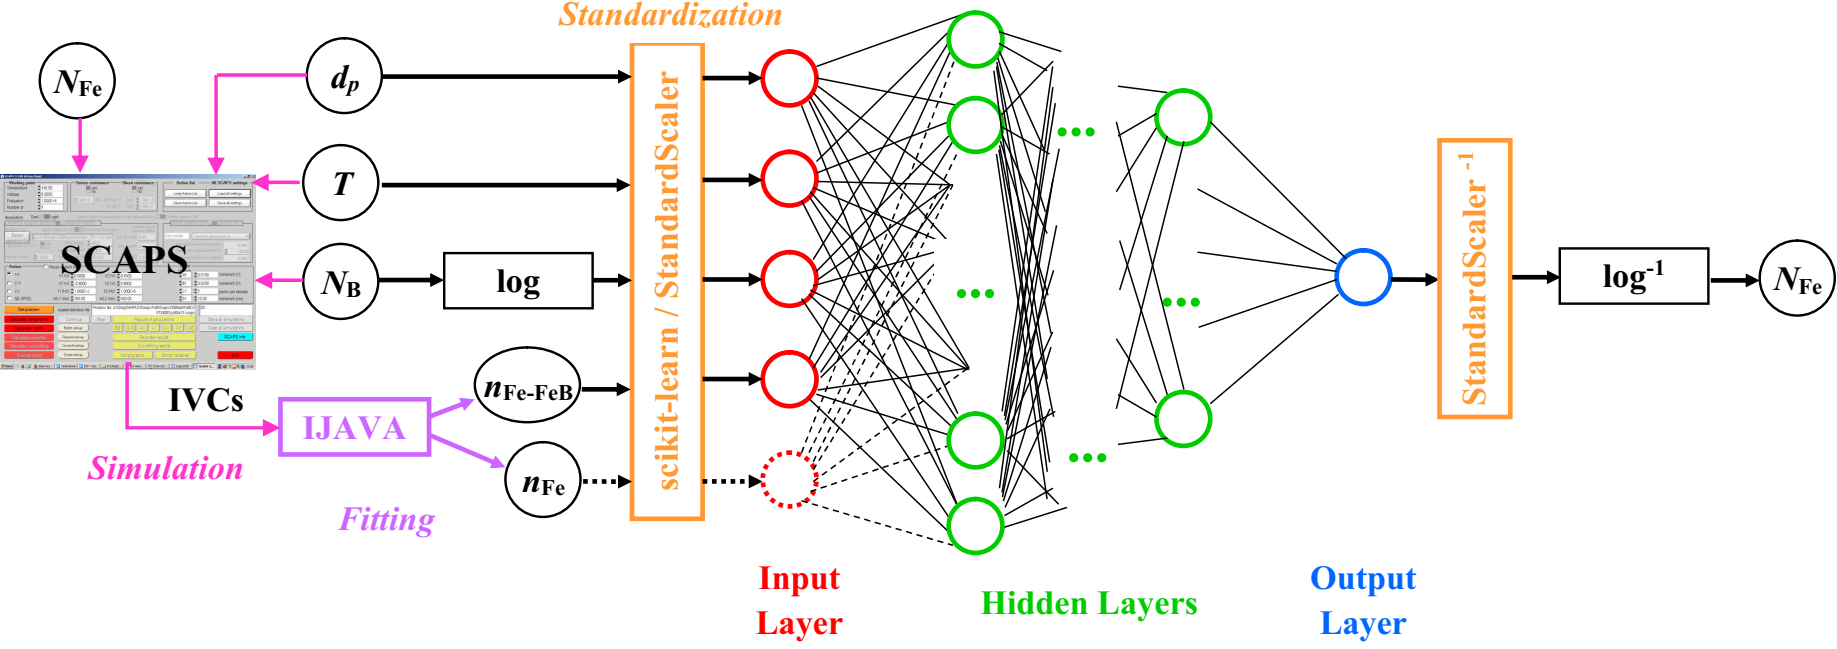
\includegraphics[width=0.9\textwidth]{Chem}
\caption{Flowchart of the work  steps.
Additional details are discussed in the body of the article.}
\label{fig_chem}
\end{figure*}


\section{Simulation Details}

\subsection{Temperature Dependencies of Material Parameters}

To receive more relevant labeled data, the IVC simulation was performed with regard to following silicon properties:
\begin{enumerate}
  \item~the bandgap temperature dependence according to P\"assler equation \cite{Pasler};
  \item~the doping induced bandgap narrowing \cite{EgNarrow};
  \item~the thermal carrier velocities from \cite{Nc:Green};
  \item~the temperature dependence of effective states density  according to \cite{Si_ni_Couderc};
  \item~the free carrier effective masses from \cite{OMara}
  \item~the carrier mobilities according to Klaassen's theory  \cite{KLAASSEN953};
  \item~the temperature and doping level dependencies of band--to--band and Auger recombination coefficients from \cite{Si_BtB} and \cite{Si_Auger} respectively.
\end{enumerate}

\subsection{Defect Parameters}

The simulation was carried out under the assumption that the defect--assisted recombination was
bound up with iron--related deep levels.
We have assumed uniform iron atom distribution in both SC base ($p$--region) and BSF--layer ($p^+$--region) with concentration $N_{\mathrm{Fe}}$.
Simulations were carried out for two cases.
In the first equilibrium one, the iron is believed to be both in the interstitial lattice position ($\mathrm{Fe}_i$) and in the trigonal pair with shallow acceptors (boron, $\mathrm{Fe}_i\mathrm{B}_s$).
The pair's fraction does not constant in SC regions and is given by \cite{MurphyJAP2011,FeB:kinetic}
\begin{equation}
\label{eqNFeB}
    \frac{N_{\mathrm{FeB}}}{N_{\mathrm{Fe}}}=\frac{N_\mathrm{B}10^{-23}\exp\left(-\frac{E_b}{kT}\right)}
     {\left[1+\frac{N_\mathrm{B}}{10^{23}}\exp\left(-\frac{E_b}{kT}\right)\right]\left[1+\exp\left(-\frac{F-E_{\mathrm{Fe}_i}}{kT}\right)\right]}\,,
\end{equation}
where
$N_\mathrm{B}$ is the boron concentration,
$F$ is the Fermi level,
$E_b=0.582$~eV is the binding energy of the $\mathrm{Fe}_i\mathrm{B}_s$ pairs,
$E_{\mathrm{Fe}_i}$ is the donor level, associated with $\mathrm{Fe}_i$.
This case referred as "Fe-FeB" hereafter.

In the second one (referred as "Fe"--case), the $\mathrm{Fe}_i$ was suggested to be only present  with uniform distribution.
Such state can be realized by heat treatment (210$^\circ$C, 3~min) \cite{FeB_Zong} or intense illumination \cite{FeBLight2}.

The donor level $E_{\mathrm{Fe}_i} = E_V+0.394$~eV
with electron $\sigma_{n,{\mathrm{Fe}}}=3.47\times10^{-11}T^{-1.48}$~cm$^2$ and
hole $\sigma_{p,{\mathrm{Fe}}}=4.54\times10^{-16}\exp\left(-\frac{0.05}{kT}\right)$~cm$^2$ capture cross-sections \cite{MurphyJAP2011,ROUGIEUX2018}
was associated with $\mathrm{Fe}_i$.
The donor level $E_{\mathrm{FeB}}^\mathrm{D}= E_V+0.10$~eV,
$\sigma_{n,{\mathrm{FeB}}}^\mathrm{D}=4\times10^{-13}$~cm$^2$,
$\sigma_{p,{\mathrm{FeB}}}^\mathrm{D}=2\times10^{-14}$~cm$^2$
and acceptor level $E_{\mathrm{FeB}}^\mathrm{A}= E_C-0.26$~eV,
$\sigma_{n,{\mathrm{FeB}}}^\mathrm{A}=5.1\times10^{-9}T^{-2.5}$~cm$^2$,
$\sigma_{p,{\mathrm{FeB}}}^\mathrm{A}=3.32\times10^{-10}\exp\left(-\frac{0.262}{kT}\right)$~cm$^2$
\cite{Istratov1999,MurphyJAP2011,ROUGIEUX2018}
were used in simulation for $\mathrm{Fe}_i\mathrm{B}_s$.

\subsection{Structure Parameters}

The dark IVCs for $n^+$--$p$--$p^+$-Si structure were simulated.
The thickness and donor concentration for emitter layer ($n^+$) were $0.5$~$\mu$m and $10^{19}$~cm$^{-3}$.
The BSF--layer with thickness  $1$~$\mu$m and acceptor concentration $5\times10^{18}$~cm$^{-3}$ was used.
The base thickness $d_p$ ($150$--$240$~$\mu$m) and doping level (boron concentration, $N_\mathrm{B}=10^{15}$--$10^{17}$~cm$^{-3}$) changed from one simulation to another.
Other varied parameters were temperature ($T=290$--$340$~K) and iron concentration ($N_{\mathrm{Fe}}=10^{10}$--$10^{13}$~cm$^{-3}$).


4 $d_p$ values, 9 $N_\mathrm{B}$ values, 11 $T$ values and 19 $N_{\mathrm{Fe}}$ values, which
evenly
(for $T$ and $d_p$ in linear scale, for $N_{\mathrm{Fe}}$ and $N_\mathrm{B}$ in logarithmic scale)
distributed over the above ranges,
 formed a kind of parameter's grid --- see Fig.~\ref{fig_ParVal}.
To obtain training dataset, 15048 IVCs were simulated in Fe-case and Fe-FeB-case for nodes of grid.

Besides IVCs were prepared for several test datasets as well.
For example, one IVCs set was simulated by using $d_p$, $N_{\mathrm{Fe}}$ and $N_\mathrm{B}$ values
from grid nodes and divergent $T$ values.
The corresponding test dataset is labeled "T-varied" from now on.
The value of $d_p$, $N_{\mathrm{Fe}}$ and $N_\mathrm{B}$ is divergent from  grig in "d-varied",
"Fe-varied" and "B-varied" dataset, respectively.
"All-varied" dataset was calculated with using all parameter values, unmatched to ones of training dataset.
%The precise parameters values are listed in  Supplementary Material.
The precise parameters values are listed in  Supplementary Material.


\begin{figure}[bt]
\centering
%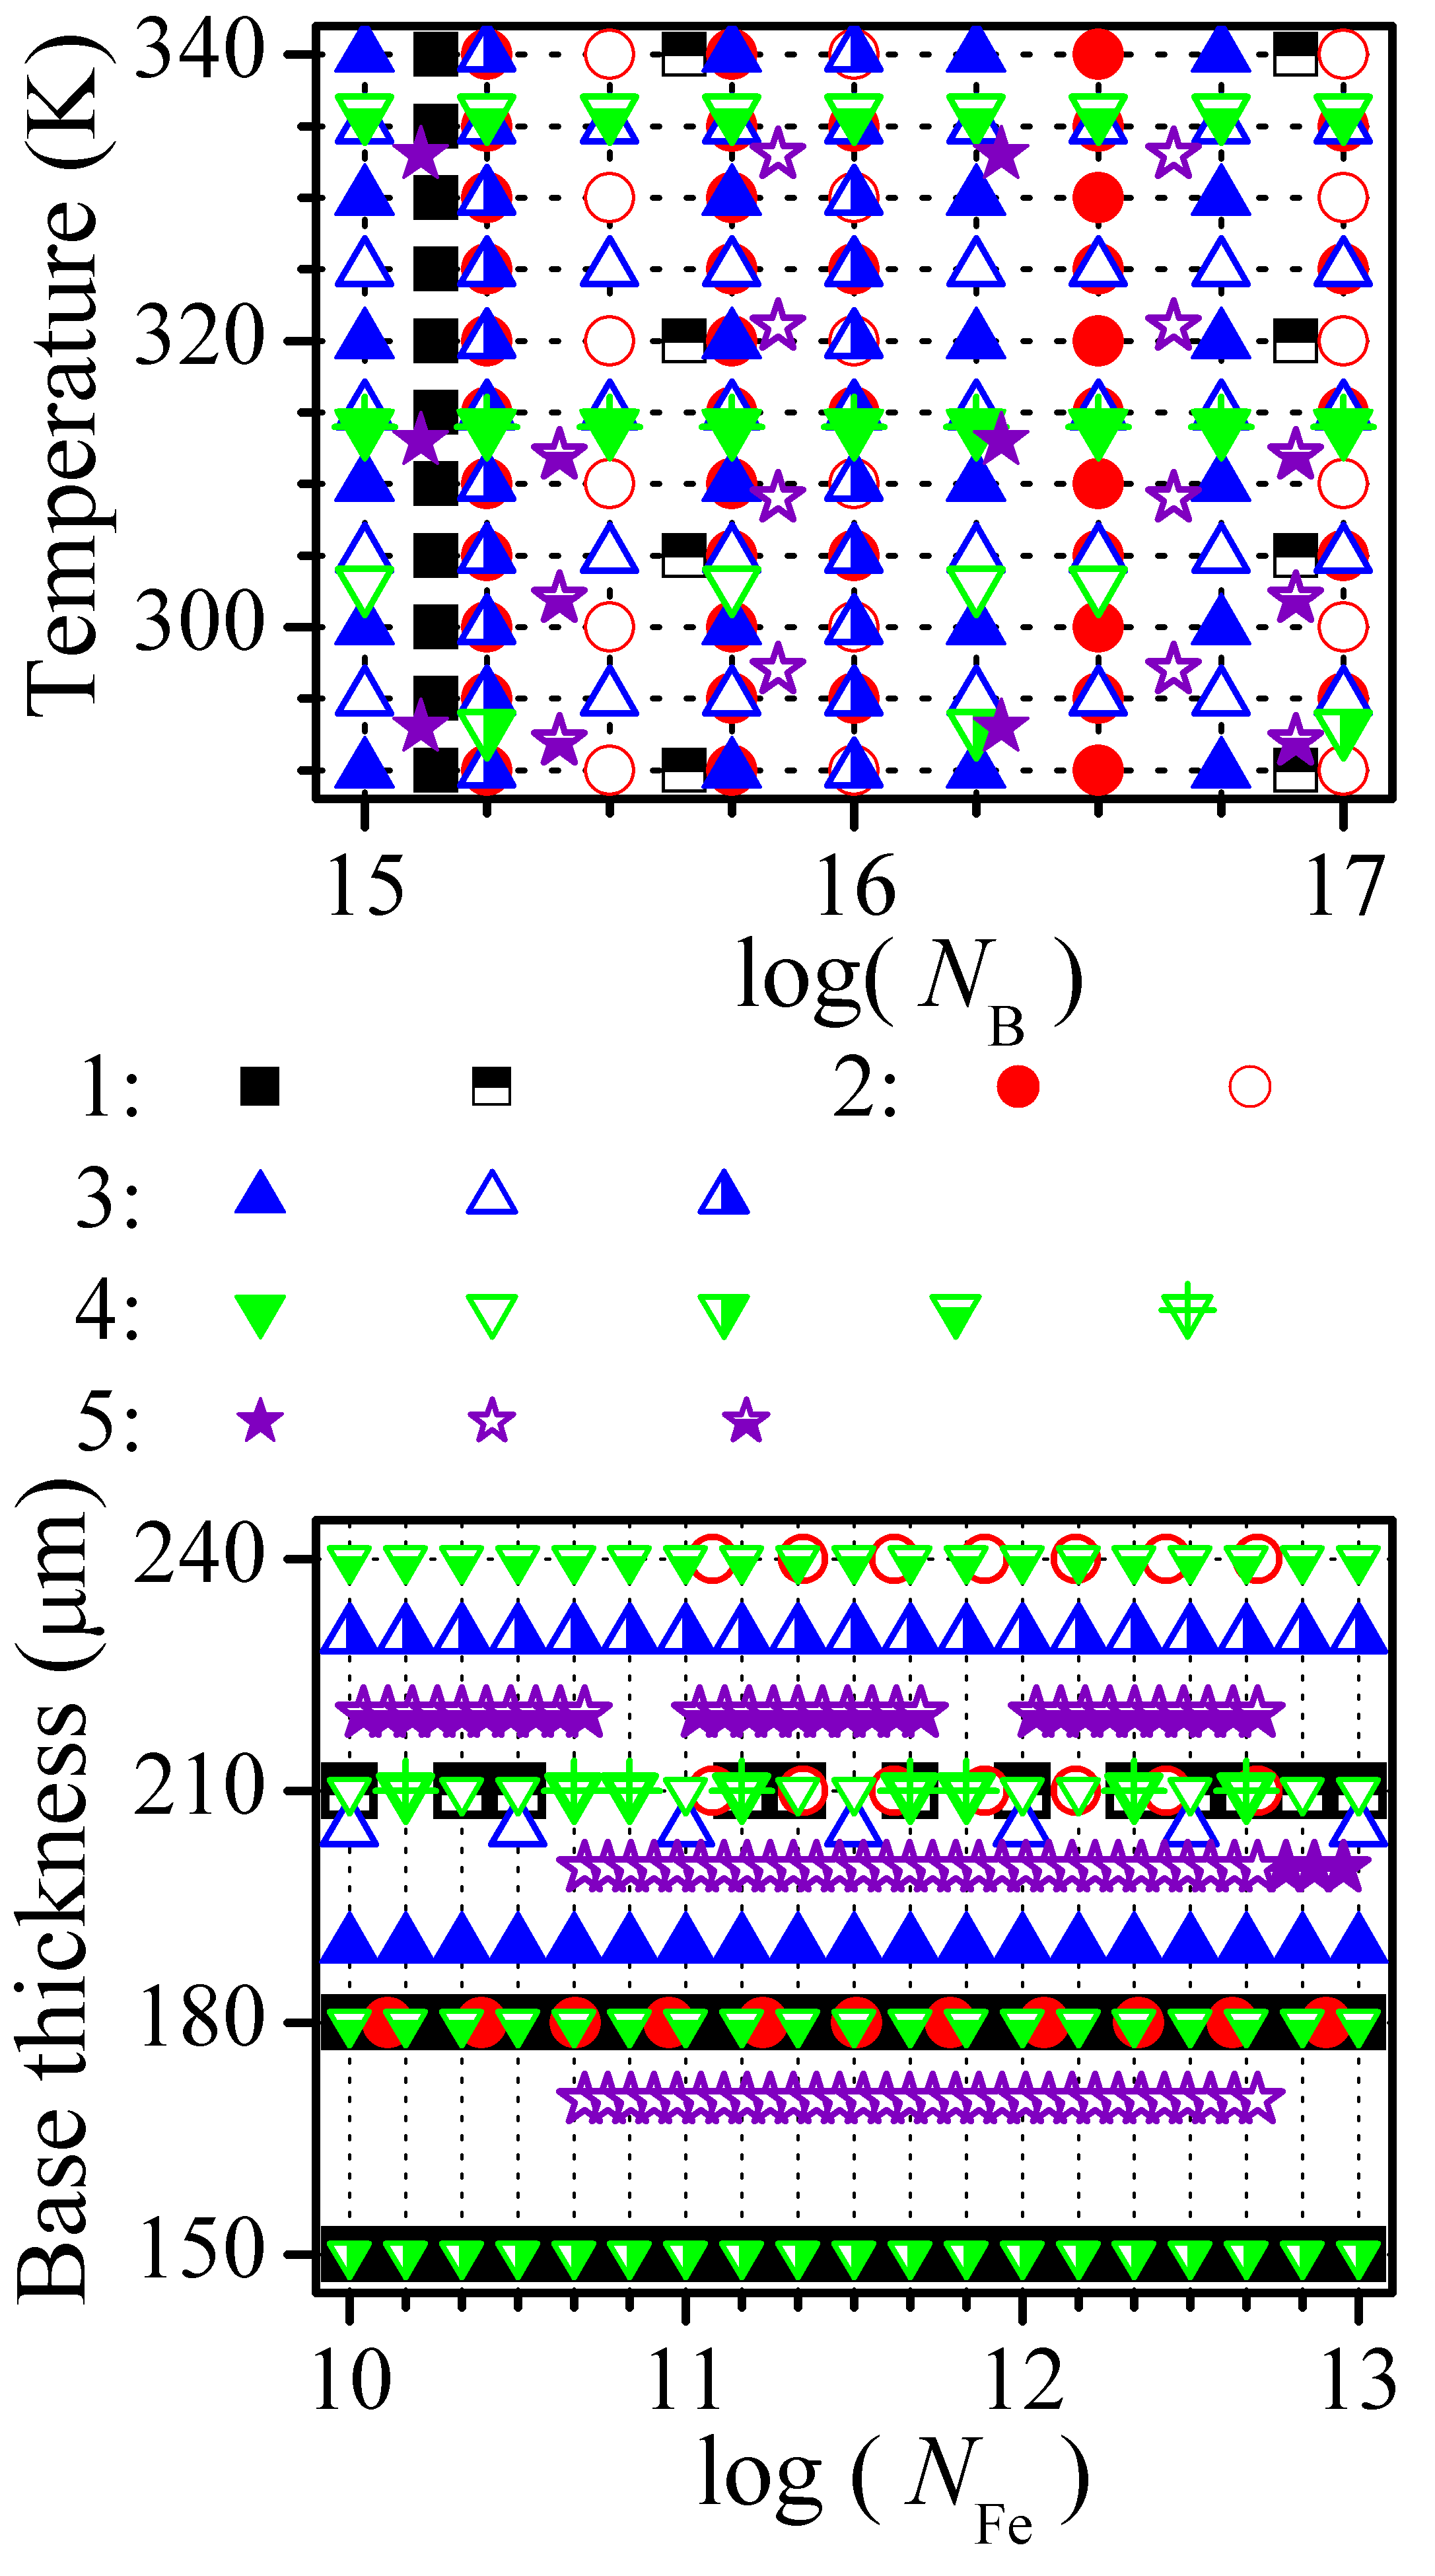
\includegraphics[width=0.3\textwidth]{FigDataAB}

\includegraphics[width=0.4\textwidth]{FigDataA}
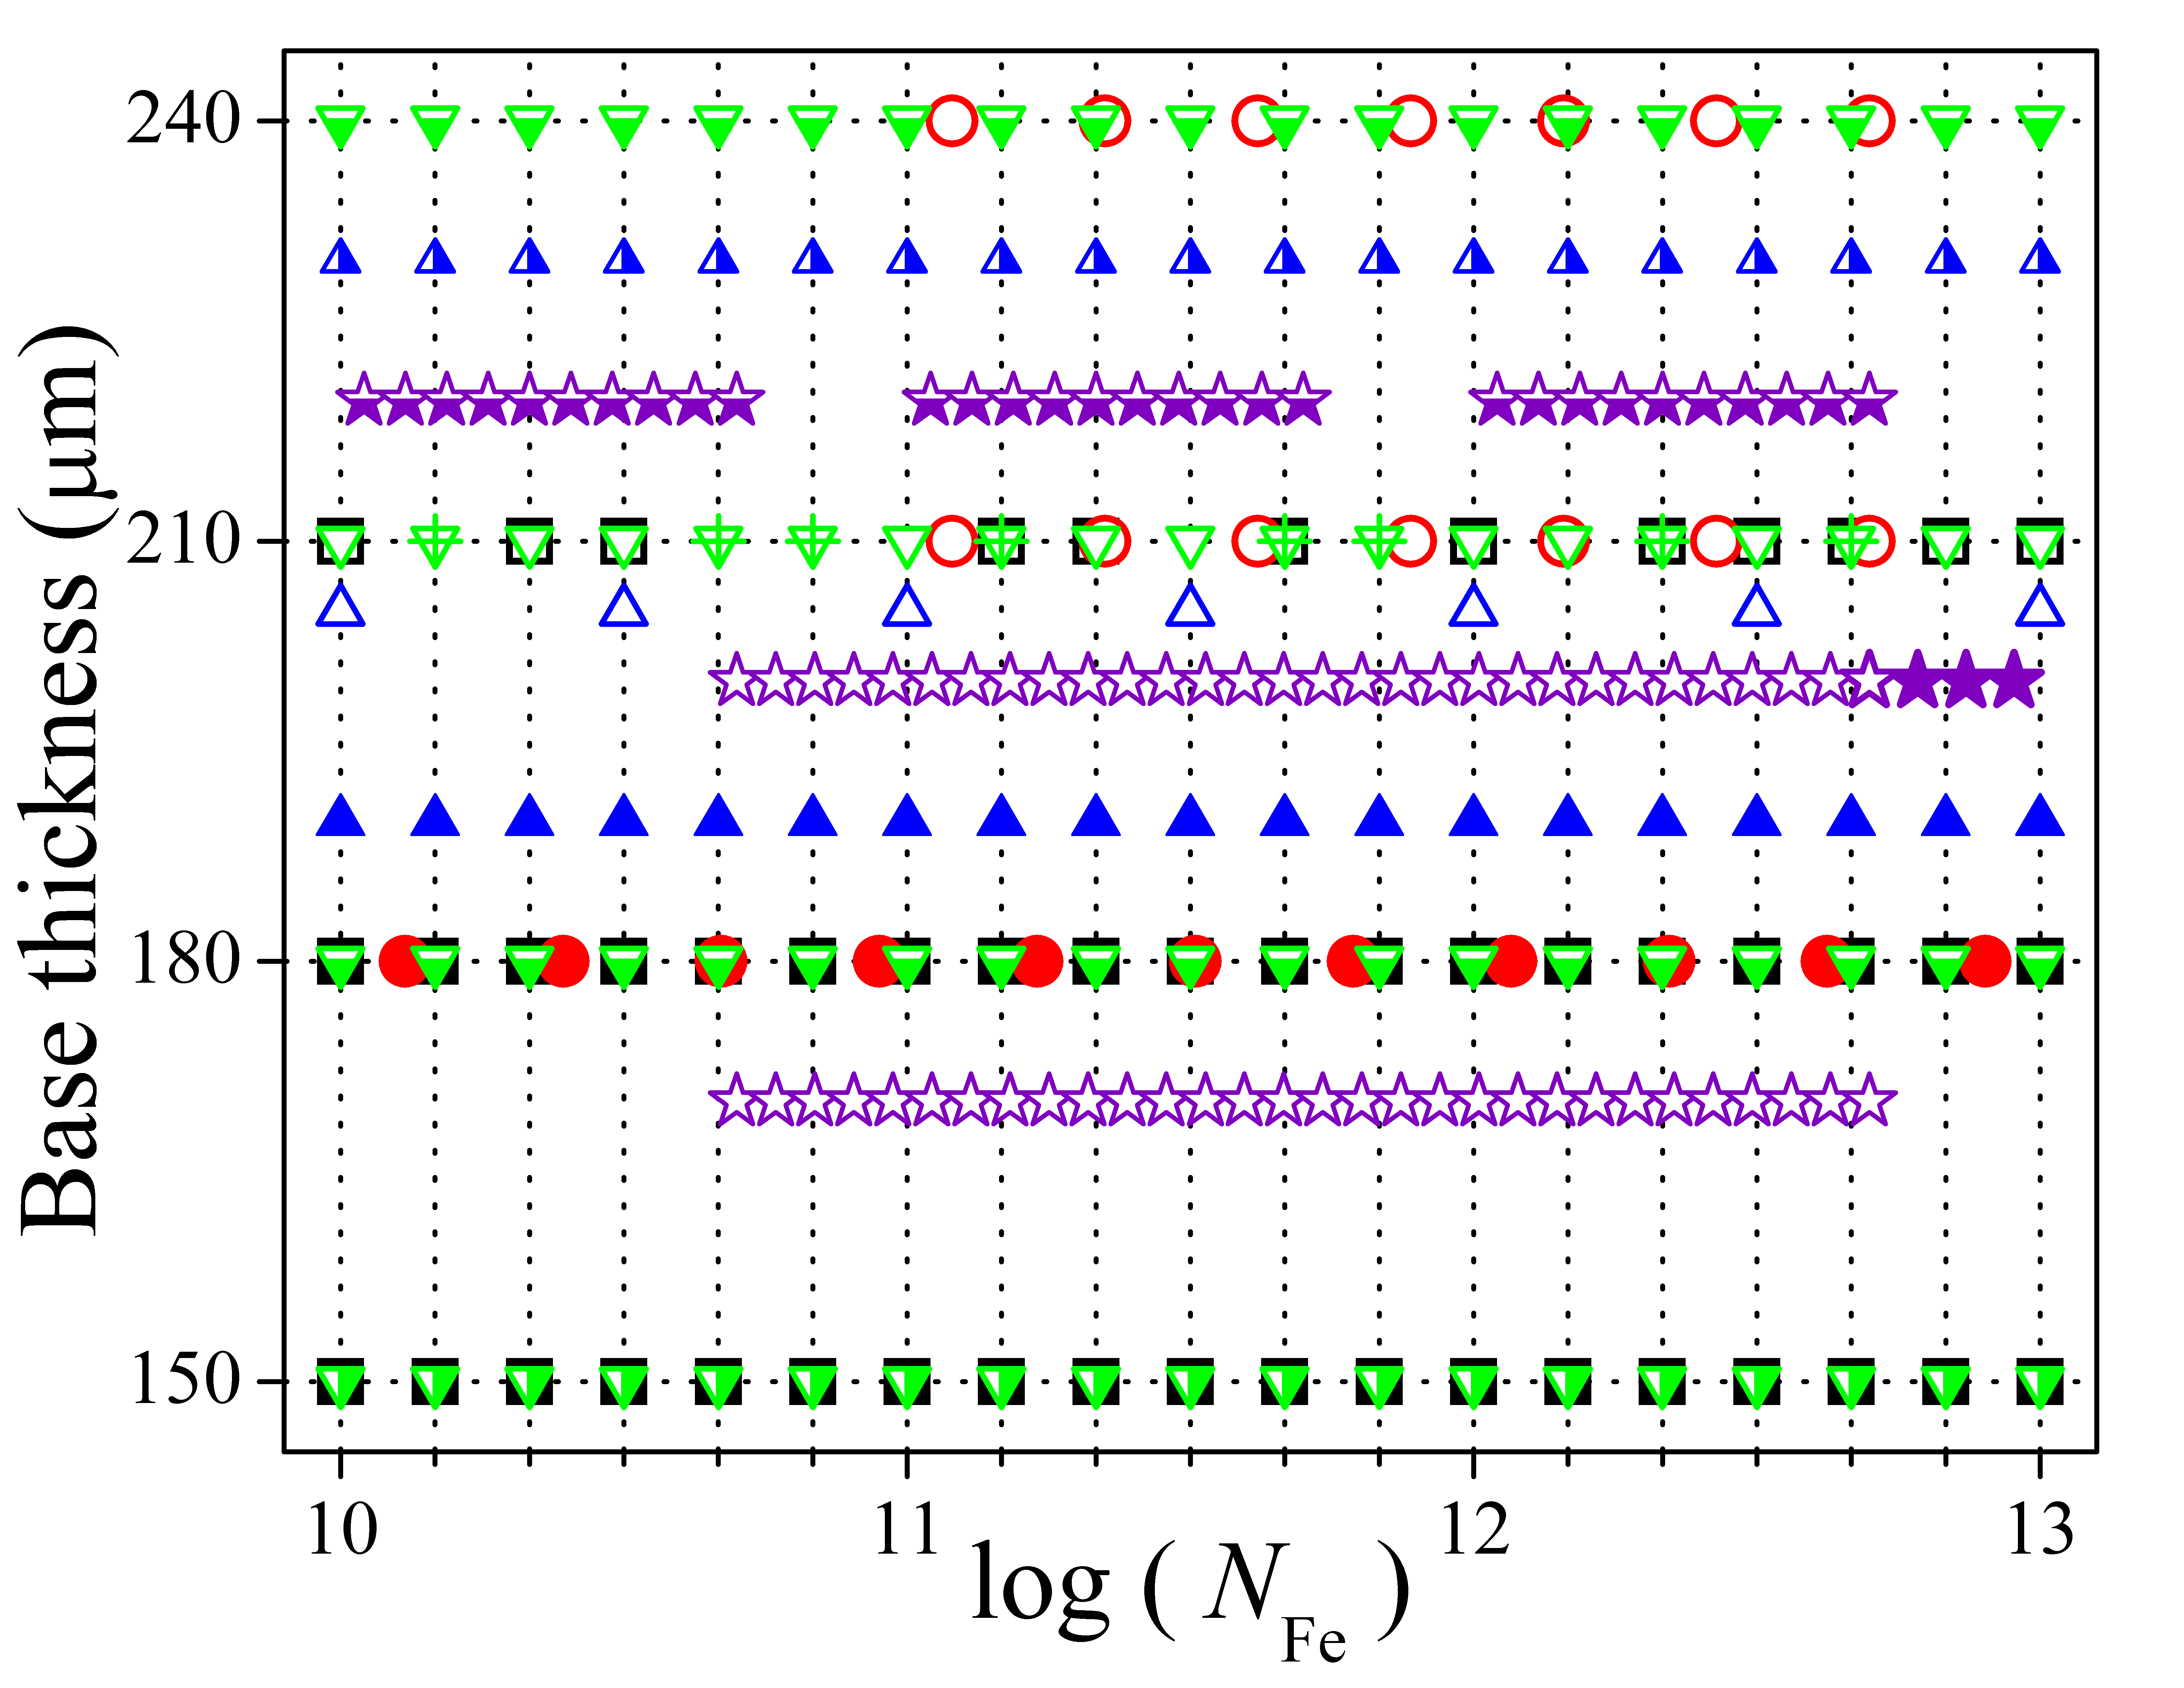
\includegraphics[width=0.4\textwidth]{FigDataB}
\caption{The parameters used for the simulations and the labeled datasets preparation.
The grid nodes and marks correspond to training dataset and test datasets
(B-varied (black squares), Fe-varied (red circles), d-varied (blue triangles up),
T-varied (green triangles down), and  All-varied (violet stars)).
Different mark interiors denote the  different subdatasets.
}
\label{fig_ParVal}
\end{figure}


\subsection{Ideality factor determination}

The simulated IVCs were fitted by using double diode model \cite{Breitenstein2013} equation
with neglecting of both series and shunt resistances:
\begin{equation}
\label{eqIV}
    I=I_{01}\left[\exp\left(-\frac{qV}{kT}\right)-1\right]+ I_{02}\left[\exp\left(-\frac{qV}{nkT}\right)-1\right]\,,
\end{equation}
%\begin{equation}
%\label{eqIV}
%    I=I_{01}\left[e^{-\frac{qV}{kT}}-1\right]+ I_{02}\left[\exp\left(-\frac{qV}{nkT}\right)-1\right]\,,
%\end{equation}
where
$I_{01}$ and $I_{02}$ are the saturation currents.
The fitting was done by using the meta--heuristic method IJAVA \cite{IJAVA}.

The ideality factor value $n_\mathrm{Fe}$ and $n_\mathrm{Fe-FeB}$ corresponds to Fe-case and Fe-FeB-case respectively.
The typical simulated dependencies of  the ideality factor are shown in Fig.~\ref{fig_nValues}.
It should be noted that $n$ can takes equal values for different parameters values
and dependencies of $n_\mathrm{Fe}$ and $n_\mathrm{Fe-FeB}$ are slightly vary.
The discussion about $n_\mathrm{Fe}$ and $n_\mathrm{Fe-FeB}$  values are presented elsewhere \cite{OlikhJPS}.


\begin{figure}[bt]
\centering
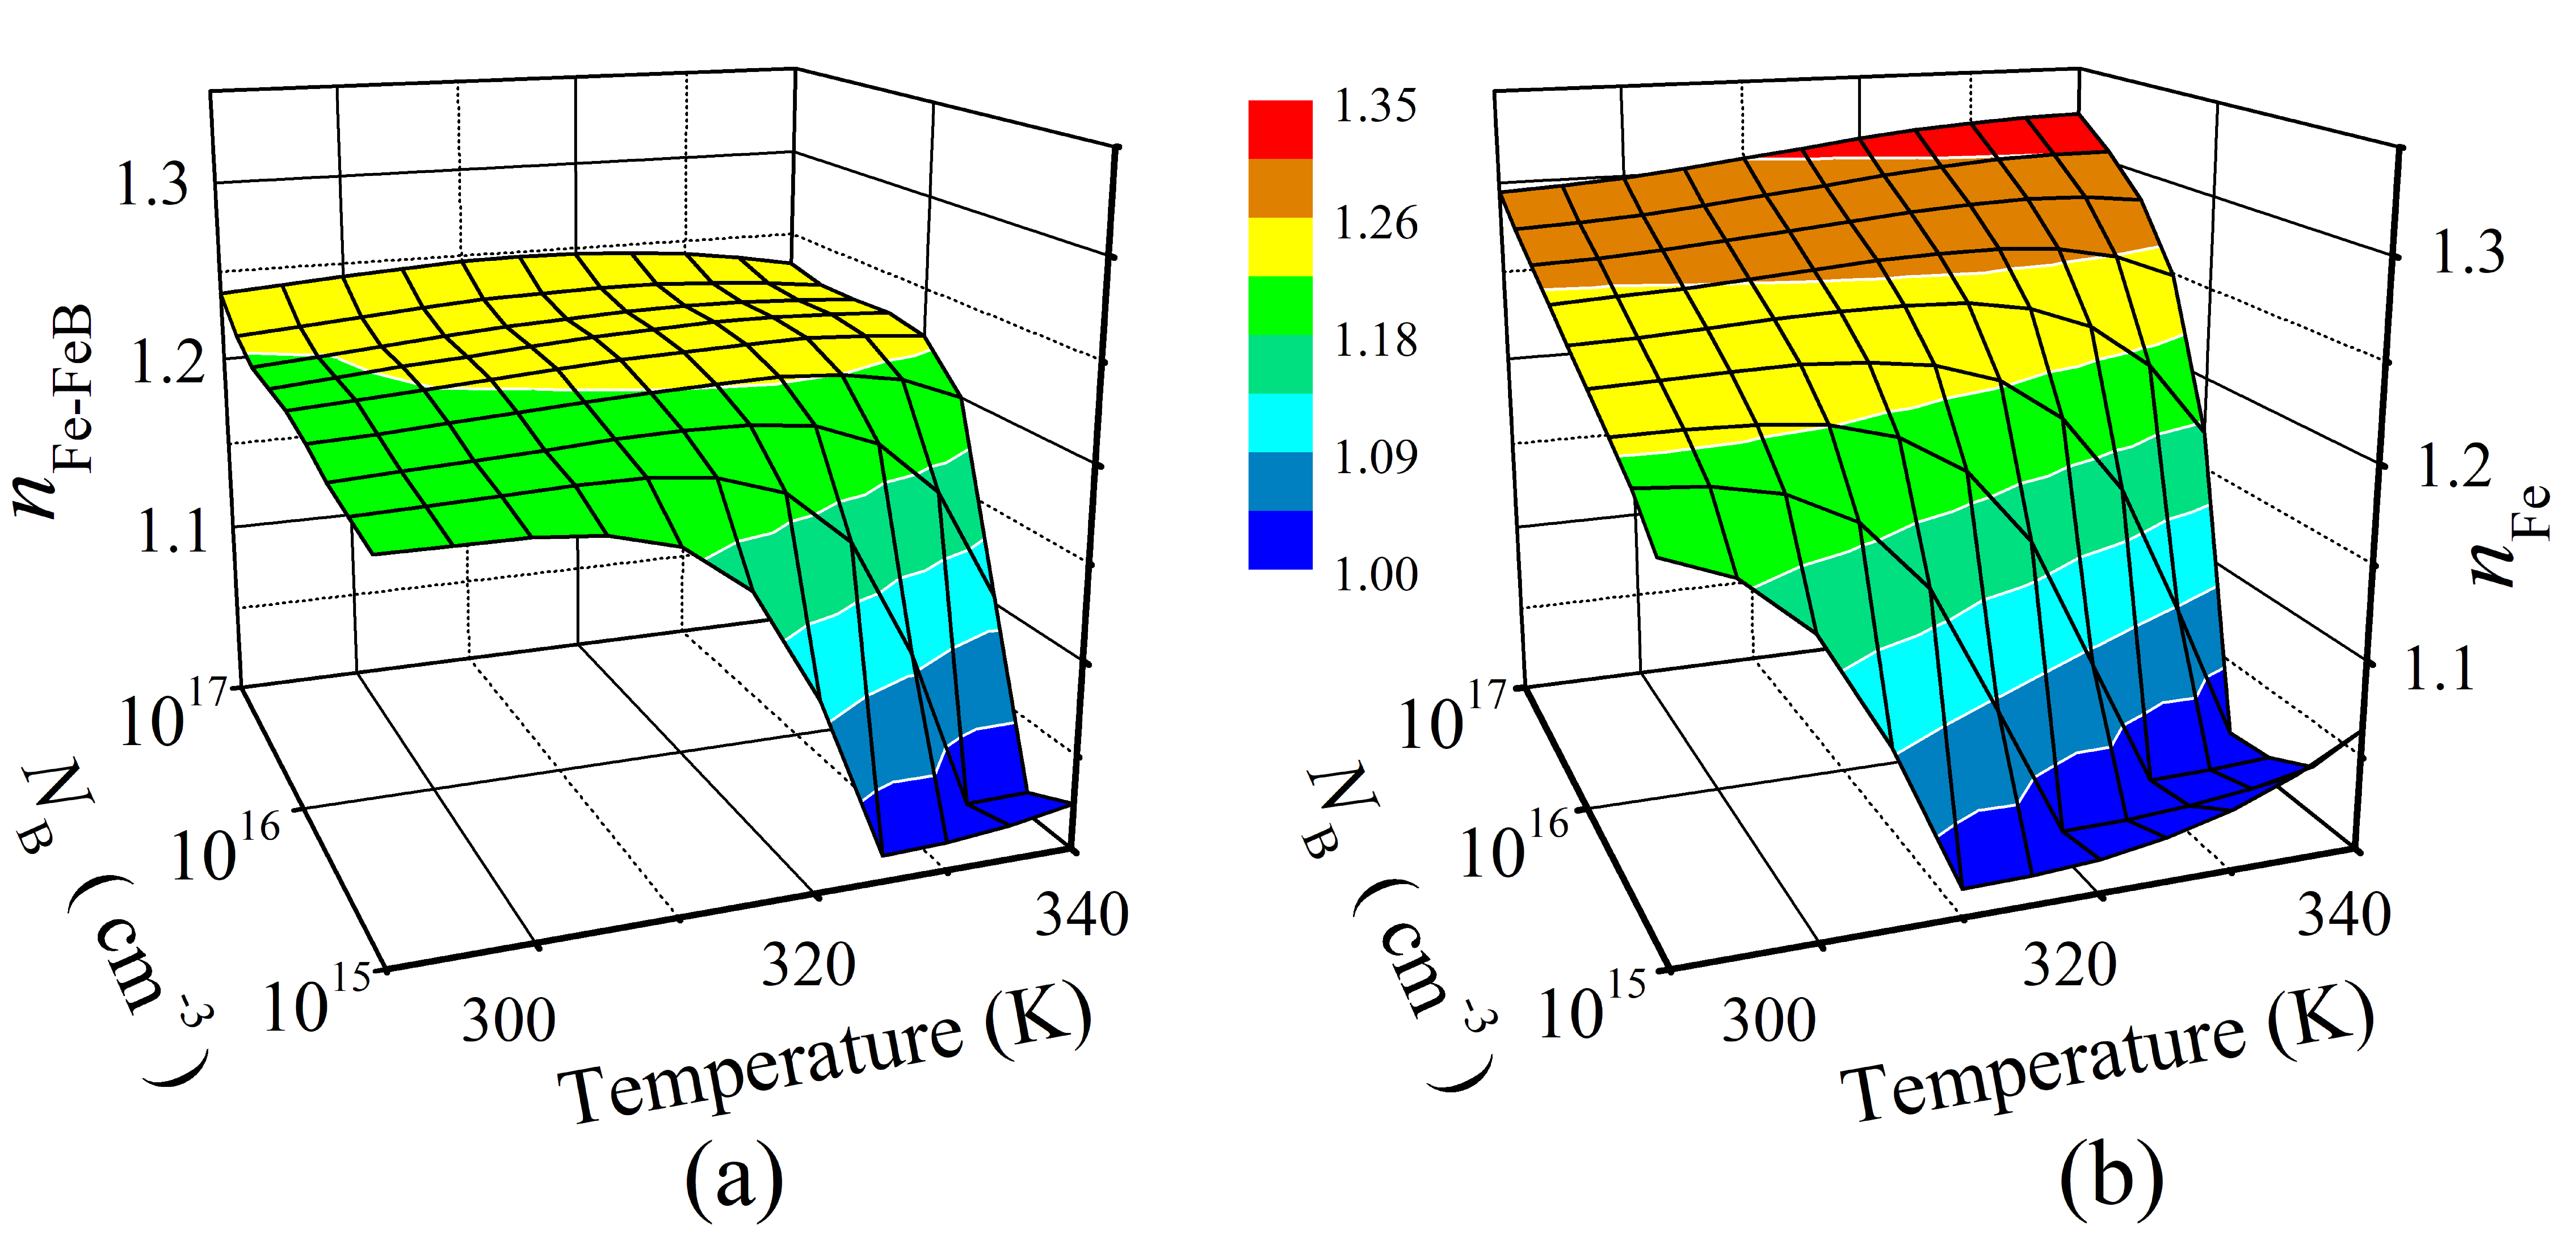
\includegraphics[width=0.5\textwidth]{Fig1a}
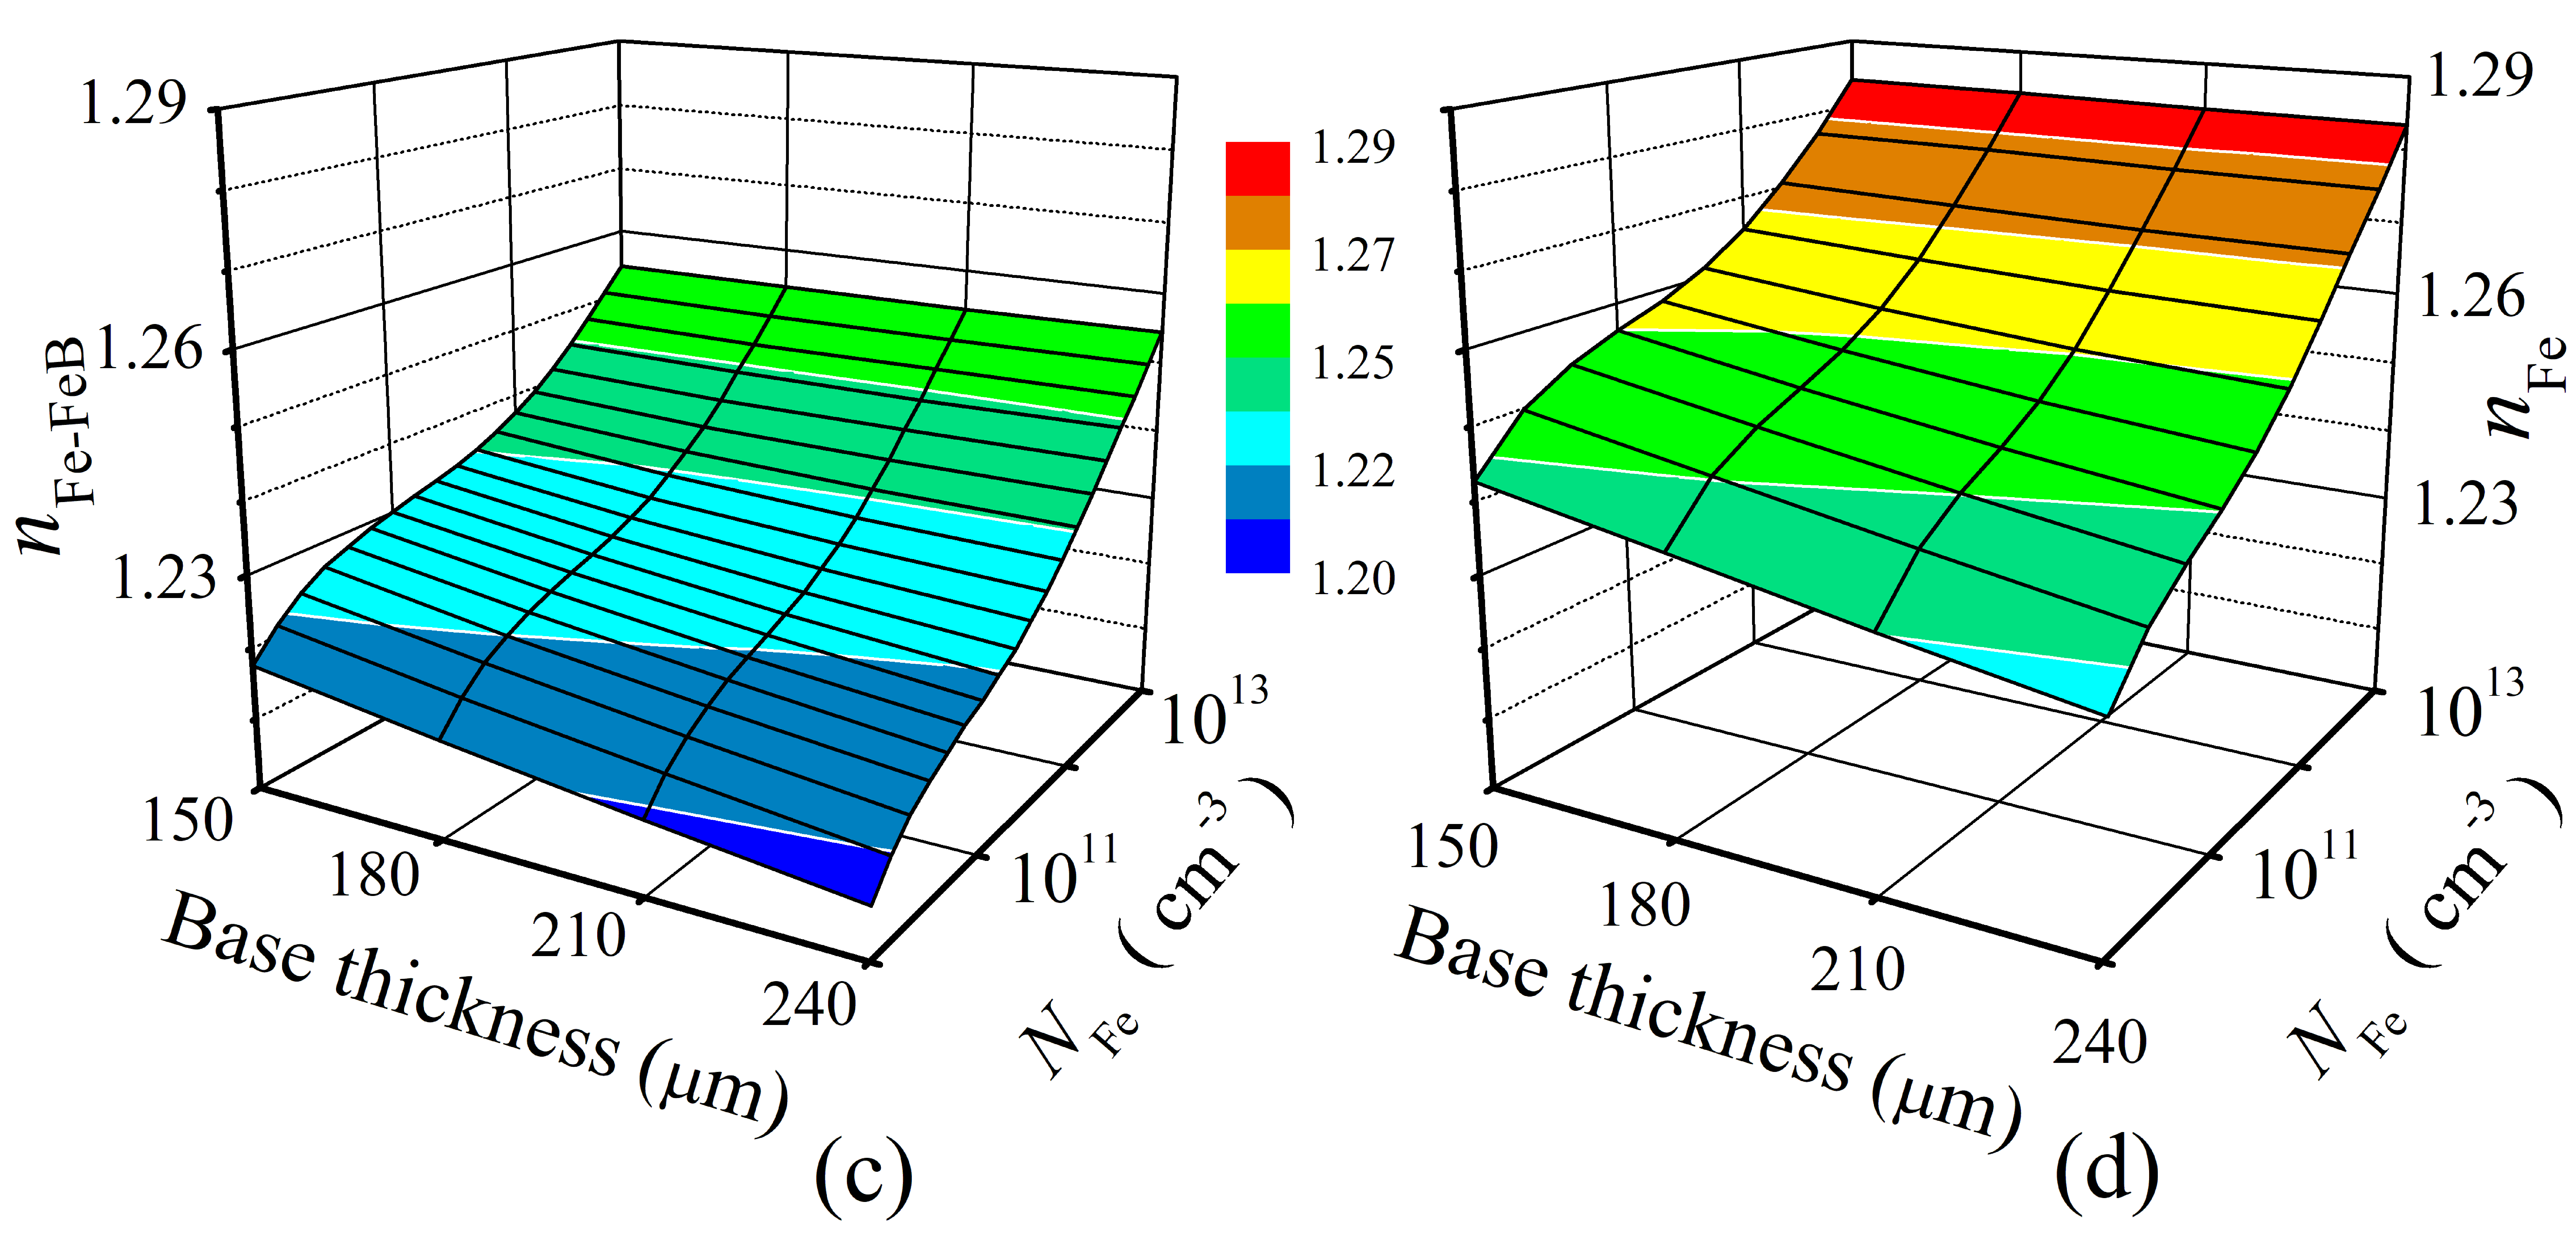
\includegraphics[width=0.5\textwidth]{Fig1b}
\caption{Ideality factor as a function of the temperature and boron concentration (a, b)
or the base thickness and iron concentration (c,d).
The cases of $\mathrm{Fe}_i\mathrm{B}_s$ and $\mathrm{Fe}_i$ coexistence (a, c)
and interstitial iron presence only (b, d).
$N_\mathrm{Fe}=10^{10}$~cm$^{-3}$ (a,b),
$d_p=180$~$\mu$m (a, b),
$N_\mathrm{B}=10^{16}$~cm$^{-3}$ (c, d),
$T=320$~K (c, d).
%Simulation results for parameter's grid are presented.
}
\label{fig_nValues}
\end{figure}


\section{Results of deep neural network using}

We have tried to construct the DNN, which is able to estimate iron contamination by using
SC parameters ($d_p$ and $N_\mathrm{B}$) and results of IVC fitting (ideality factor value)
taking into account the measurement temperature.
In one case, the result of only one dark IV measurement was used and the
set of DNN input parameters (one DNN--sample) consisted of $\{d_p,N_\mathrm{B},T,n_\mathrm{Fe-FeB}\}$.
Such case can be easy realized in practice
and corresponding neural network referred as $n_\mathrm{Fe-FeB}$ DNN hereafter.
In another case the set $\{d_p,N_\mathrm{B},T,n_\mathrm{Fe-FeB},n_\mathrm{Fe}\}$ was used in DNN input.
In practice terms, the obtaining of such a set requires additional SC processing (e.g. intense illumination) and two IV measuring.
The label $n_\mathrm{Fe-FeB}$--$n_\mathrm{Fe}$ DNN is used below.

The DNN's flowchart is shown on Fig.~\ref{fig_chem}.
The Keras API \cite{Keras} was used to set up DNN with dense layers.
Four hidden  layers with 300, 100, 30 and 30 nodes were selected.
The activation function was chosen to be Relu.
The learning rate, batch size and number of epochs were kept at 0.01, 8 and 1000 respectively.
$\log N_\mathrm{B}$ and $\log N_\mathrm{Fe}$ were used instead
$N_\mathrm{B}$ and $N_\mathrm{Fe}$ in DNN training and testing.
Standardization of a dataset was done by using \emph{StandardScaler} from \emph{scikit-learn}
(mean $=0$, standard deviation  $=1$).
The loss function was chosen mean square relative error (MSRE):
\begin{equation}
\label{eqMSRE}
    \mathrm{MSRE}=\frac{1}{N_s}\sum_{i=1}^{N_s}\frac{(N_\mathrm{Fe,TRUE,i}-N_\mathrm{Fe,PRED,i})^2}{N_\mathrm{Fe,TRUE,i}\cdot N_\mathrm{Fe,PRED,i}}\,,
\end{equation}
where
$N_s$ is the number of samples in dataset,
$N_\mathrm{Fe,TRUE,i}$ is the iron concentration, which used for simulation of $i$--th sample,
$N_\mathrm{Fe,PRED,i}$ is the DNN prediction for $i$--th sample.


10--fold cross--validation was used to estimate DNN training.
The results are listed in Table~\ref{table_CV}.
One can see that $n_\mathrm{Fe-FeB}$--$n_\mathrm{Fe}$ DNN
shows much better results.



\begin{table}[!t]
\renewcommand{\arraystretch}{1.3}
\caption{Results of 10--Fold Cross--Validation}
\label{table_CV}
\centering
\begin{tabular}{lcc}
\hline
Dataset & \multicolumn{2}{c}{MSRE}\\
%$n_\mathrm{Fe-FeB}$ DNN &$n_\mathrm{Fe-FeB}$--$n_\mathrm{Fe}$ DNN\\
 & $n_\mathrm{Fe-FeB}$ DNN &$n_\mathrm{Fe-FeB}$--$n_\mathrm{Fe}$ DNN\\
\hline
training&$0.29\pm0.07$&$0.09\pm0.04$ \\
full&$0.30\pm0.08$& $0.05\pm0.02$\\
\hline
\end{tabular}
\end{table}

DNNs, trained by parameters grid nodes data, were applied to test datasets.
Results are presented in Fig.~\ref{fig_TrPr} (a)-(e), (g)-(k) and in Table~\ref{table_MSRE}.
As it is shown, the $n_\mathrm{Fe-FeB}$ DNN can be quite wrong for some samples
($\{d_p,N_\mathrm{B},T,n_\mathrm{Fe-FeB}\}$ sets).
The largest errors are observed for doping level values, which unused during  network learning
(B-varied dataset, Fig.~\ref{fig_TrPr}(c)).
On the other hand, the variation in $N_\mathrm{Fe}$ value are well detected even $n_\mathrm{Fe-FeB}$ DNN:
$\mathrm{MSRE}=0.06$ only and SRE does not exceed 0.01 for 90\% of samples (see lines in Fig.~\ref{fig_TrPr}(d)).

\begin{table}[!t]
\renewcommand{\arraystretch}{1.3}
\caption{A Mean Square Relative Error Of
DNNs on Test Dataset}
\label{table_MSRE}
\centering
\begin{tabular}{lcc}
\hline
Dataset & $n_\mathrm{Fe-FeB}$ DNN &$n_\mathrm{Fe-FeB}$--$n_\mathrm{Fe}$ DNN\\
\hline
T--varied&0.46 & 0.06\\
B--varied&1.2 & 0.25\\
d--varied&0.36 & 0.06\\
Fe--varied&0.06 & 0.03\\
All--varied&0.49 & 0.10\\
\hline
\end{tabular}
\end{table}




\begin{figure*}[tb]
\centering
%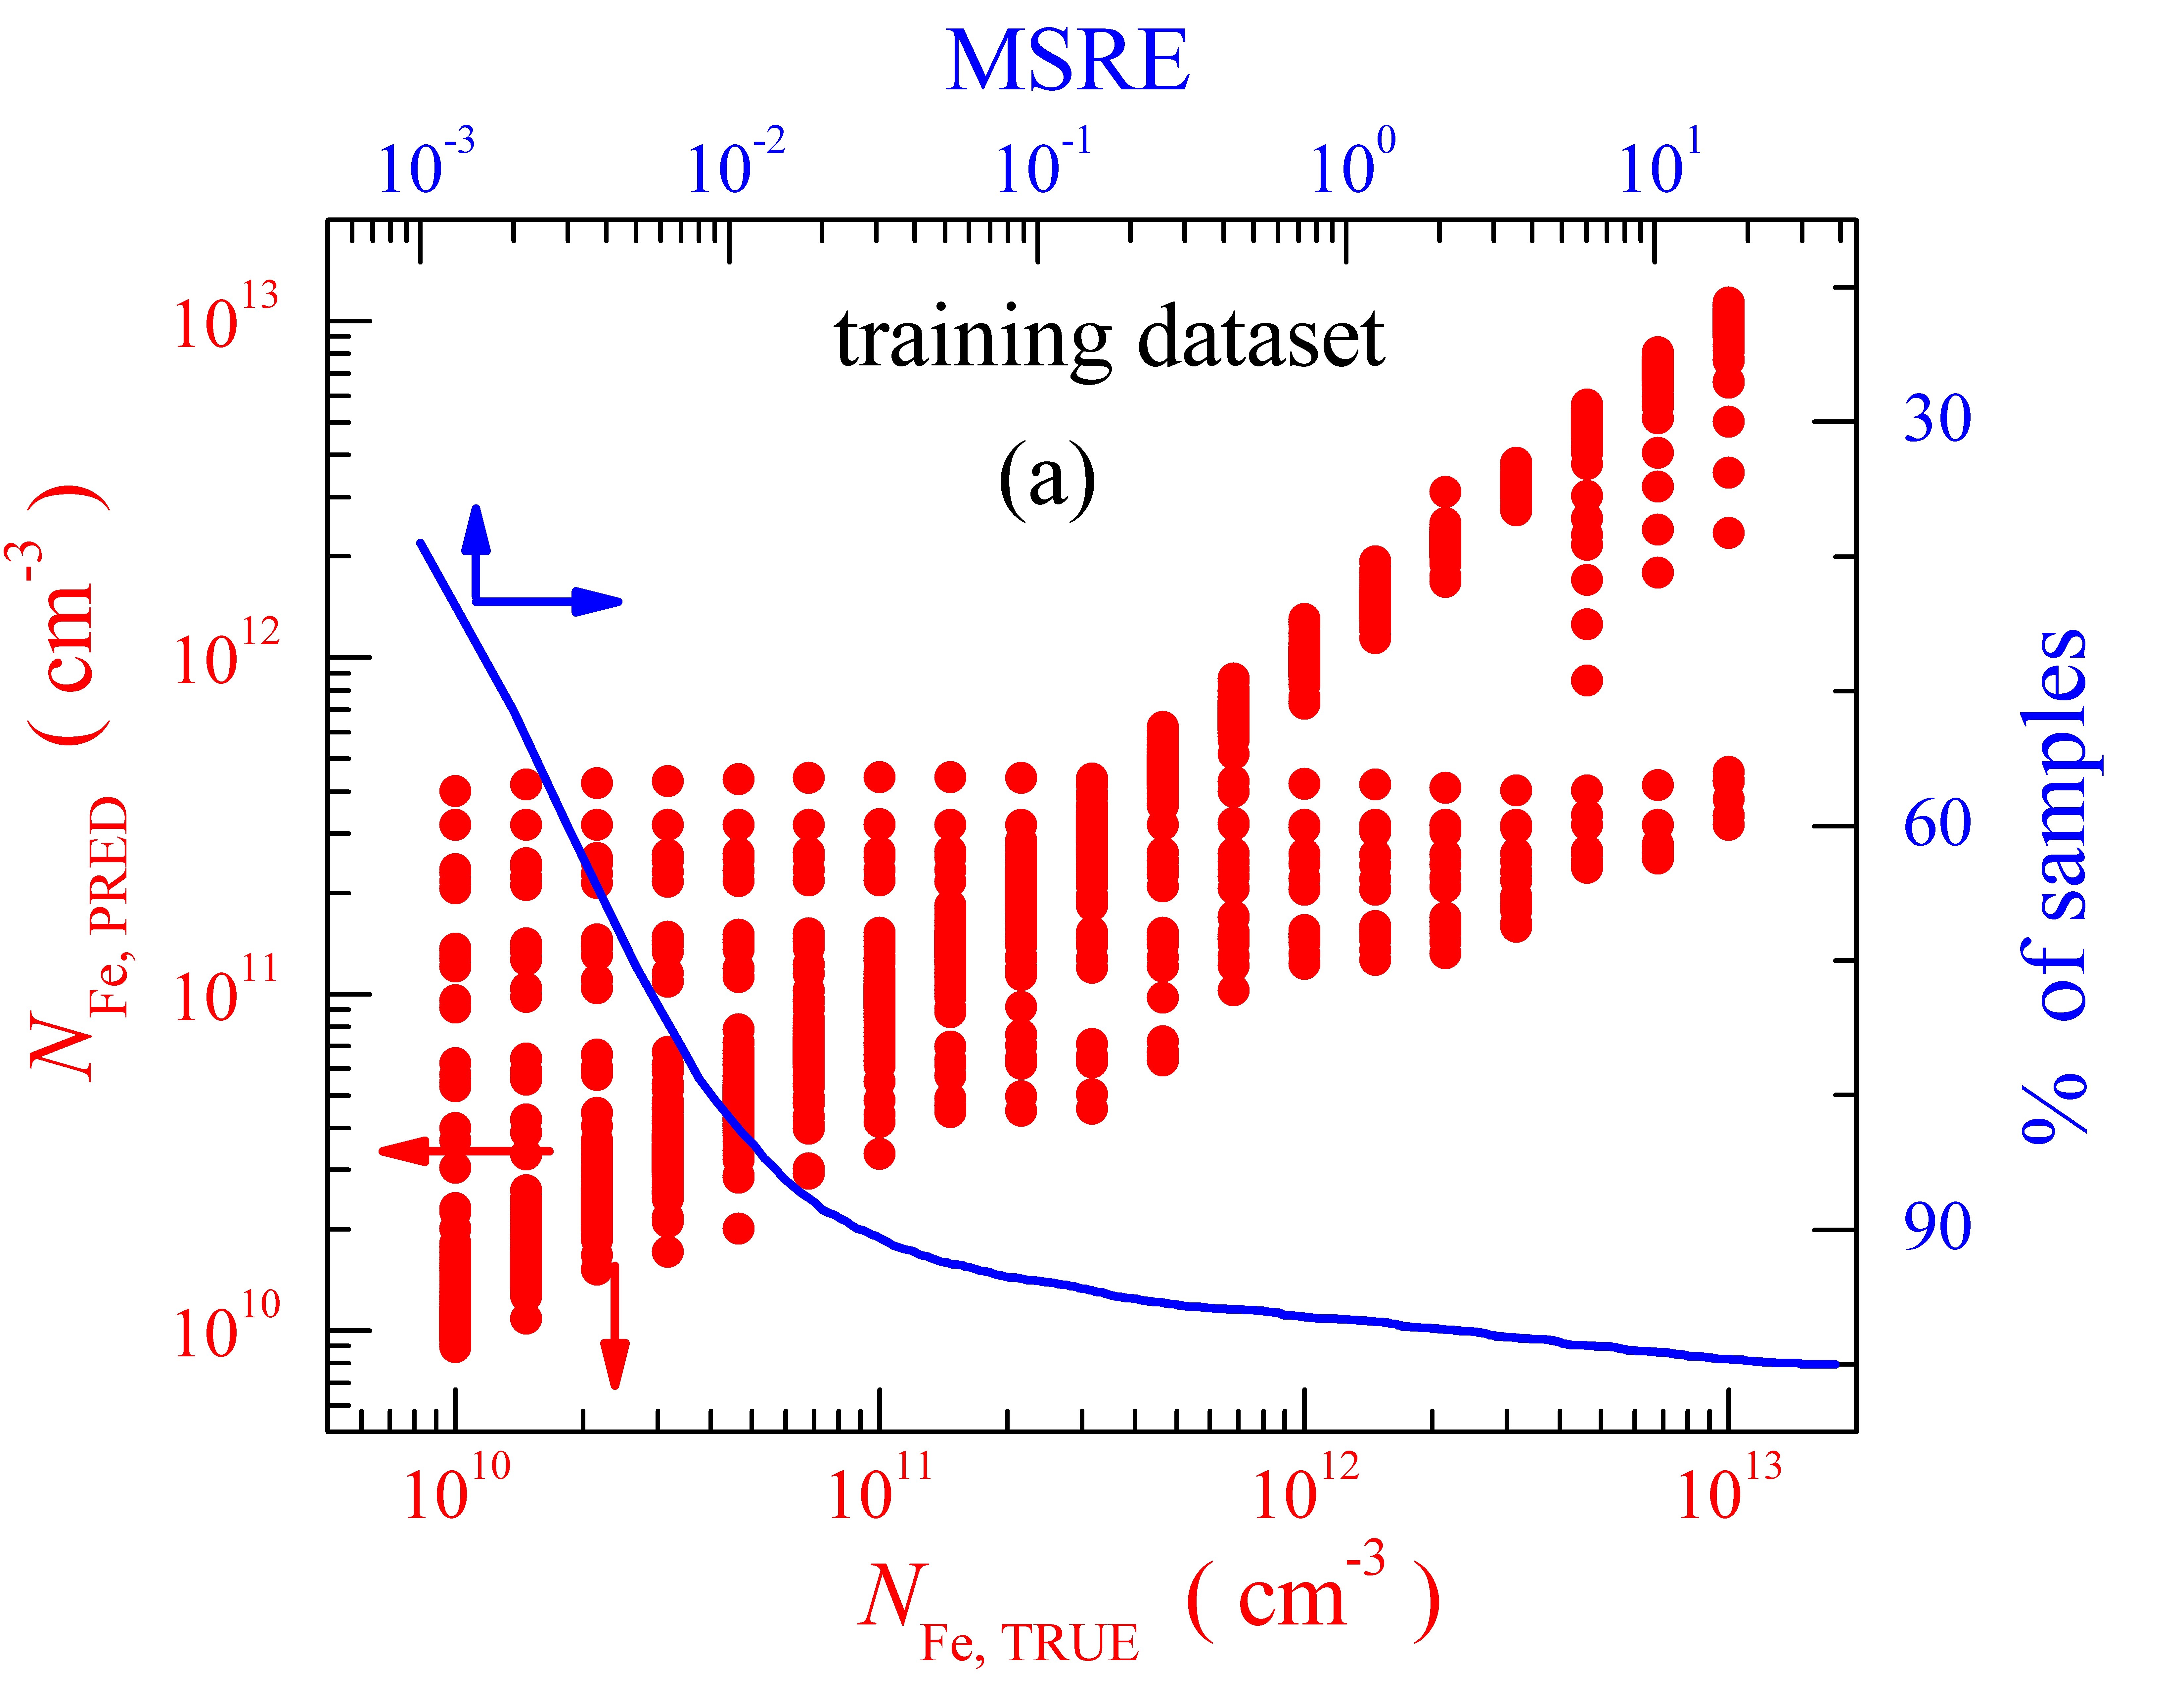
\includegraphics[width=0.32\textwidth]{Fig2a}
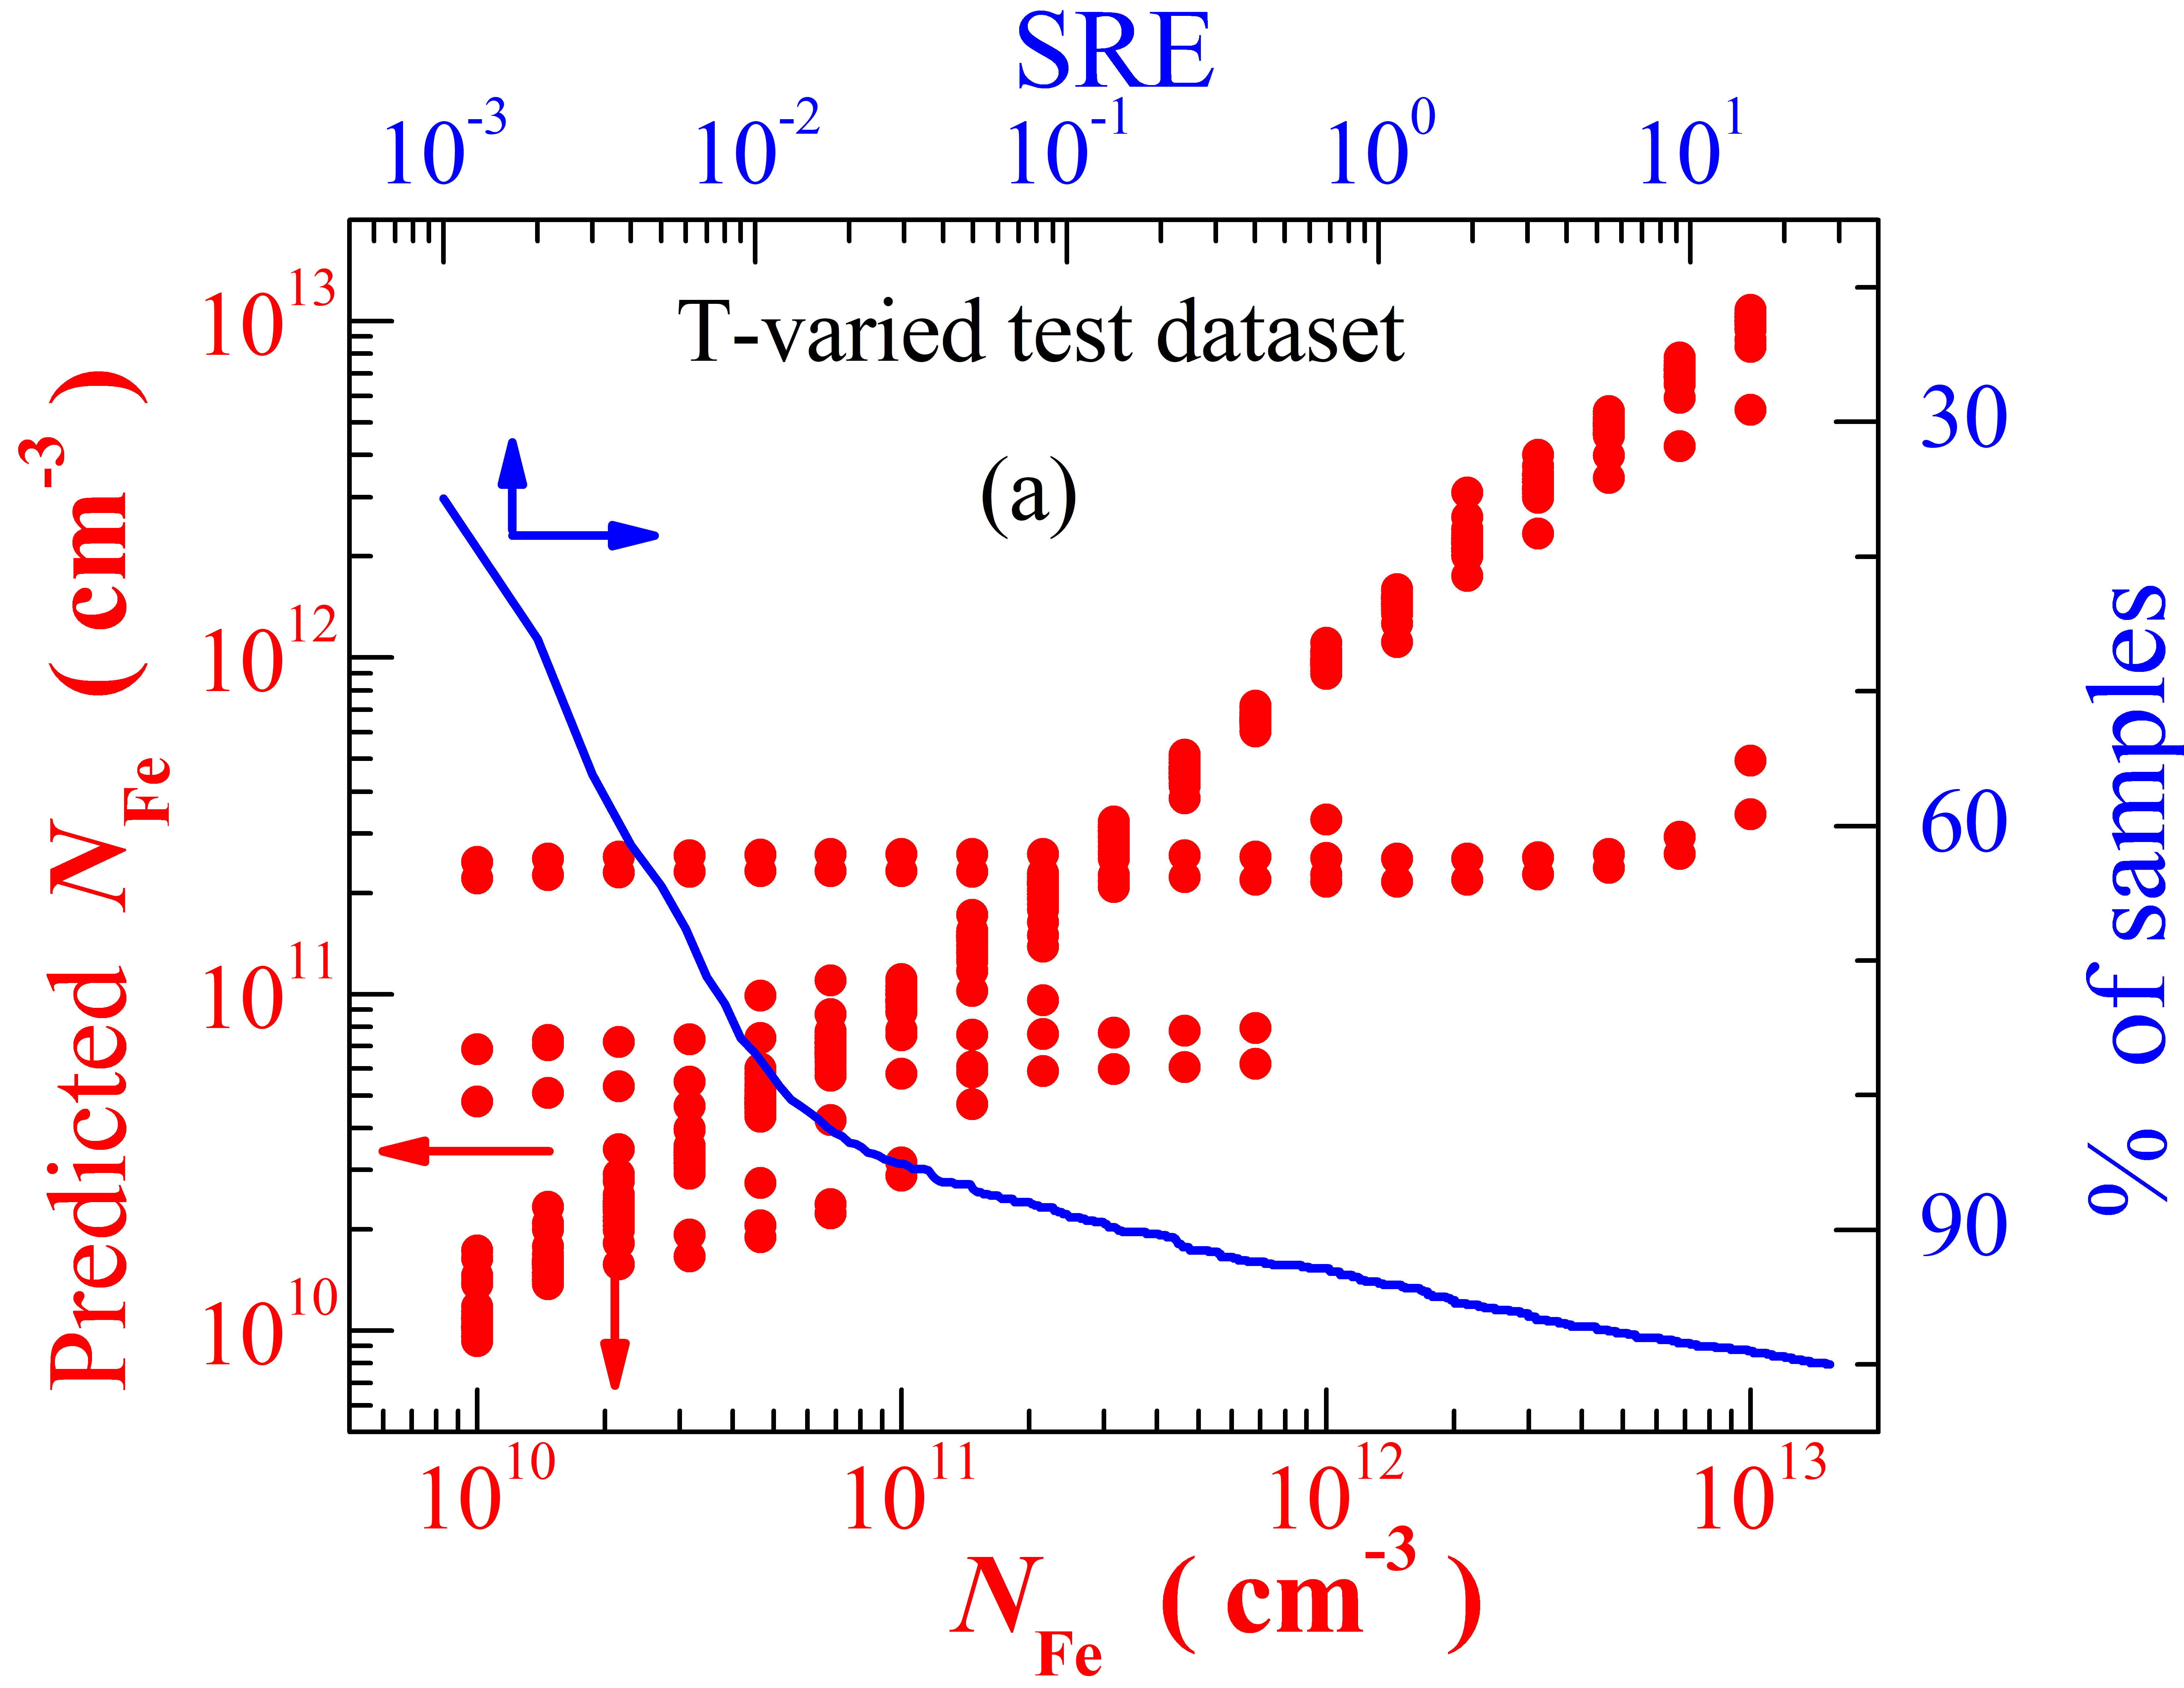
\includegraphics[width=0.32\textwidth]{Fig2b}

\includegraphics[width=0.32\textwidth]{Fig2c}
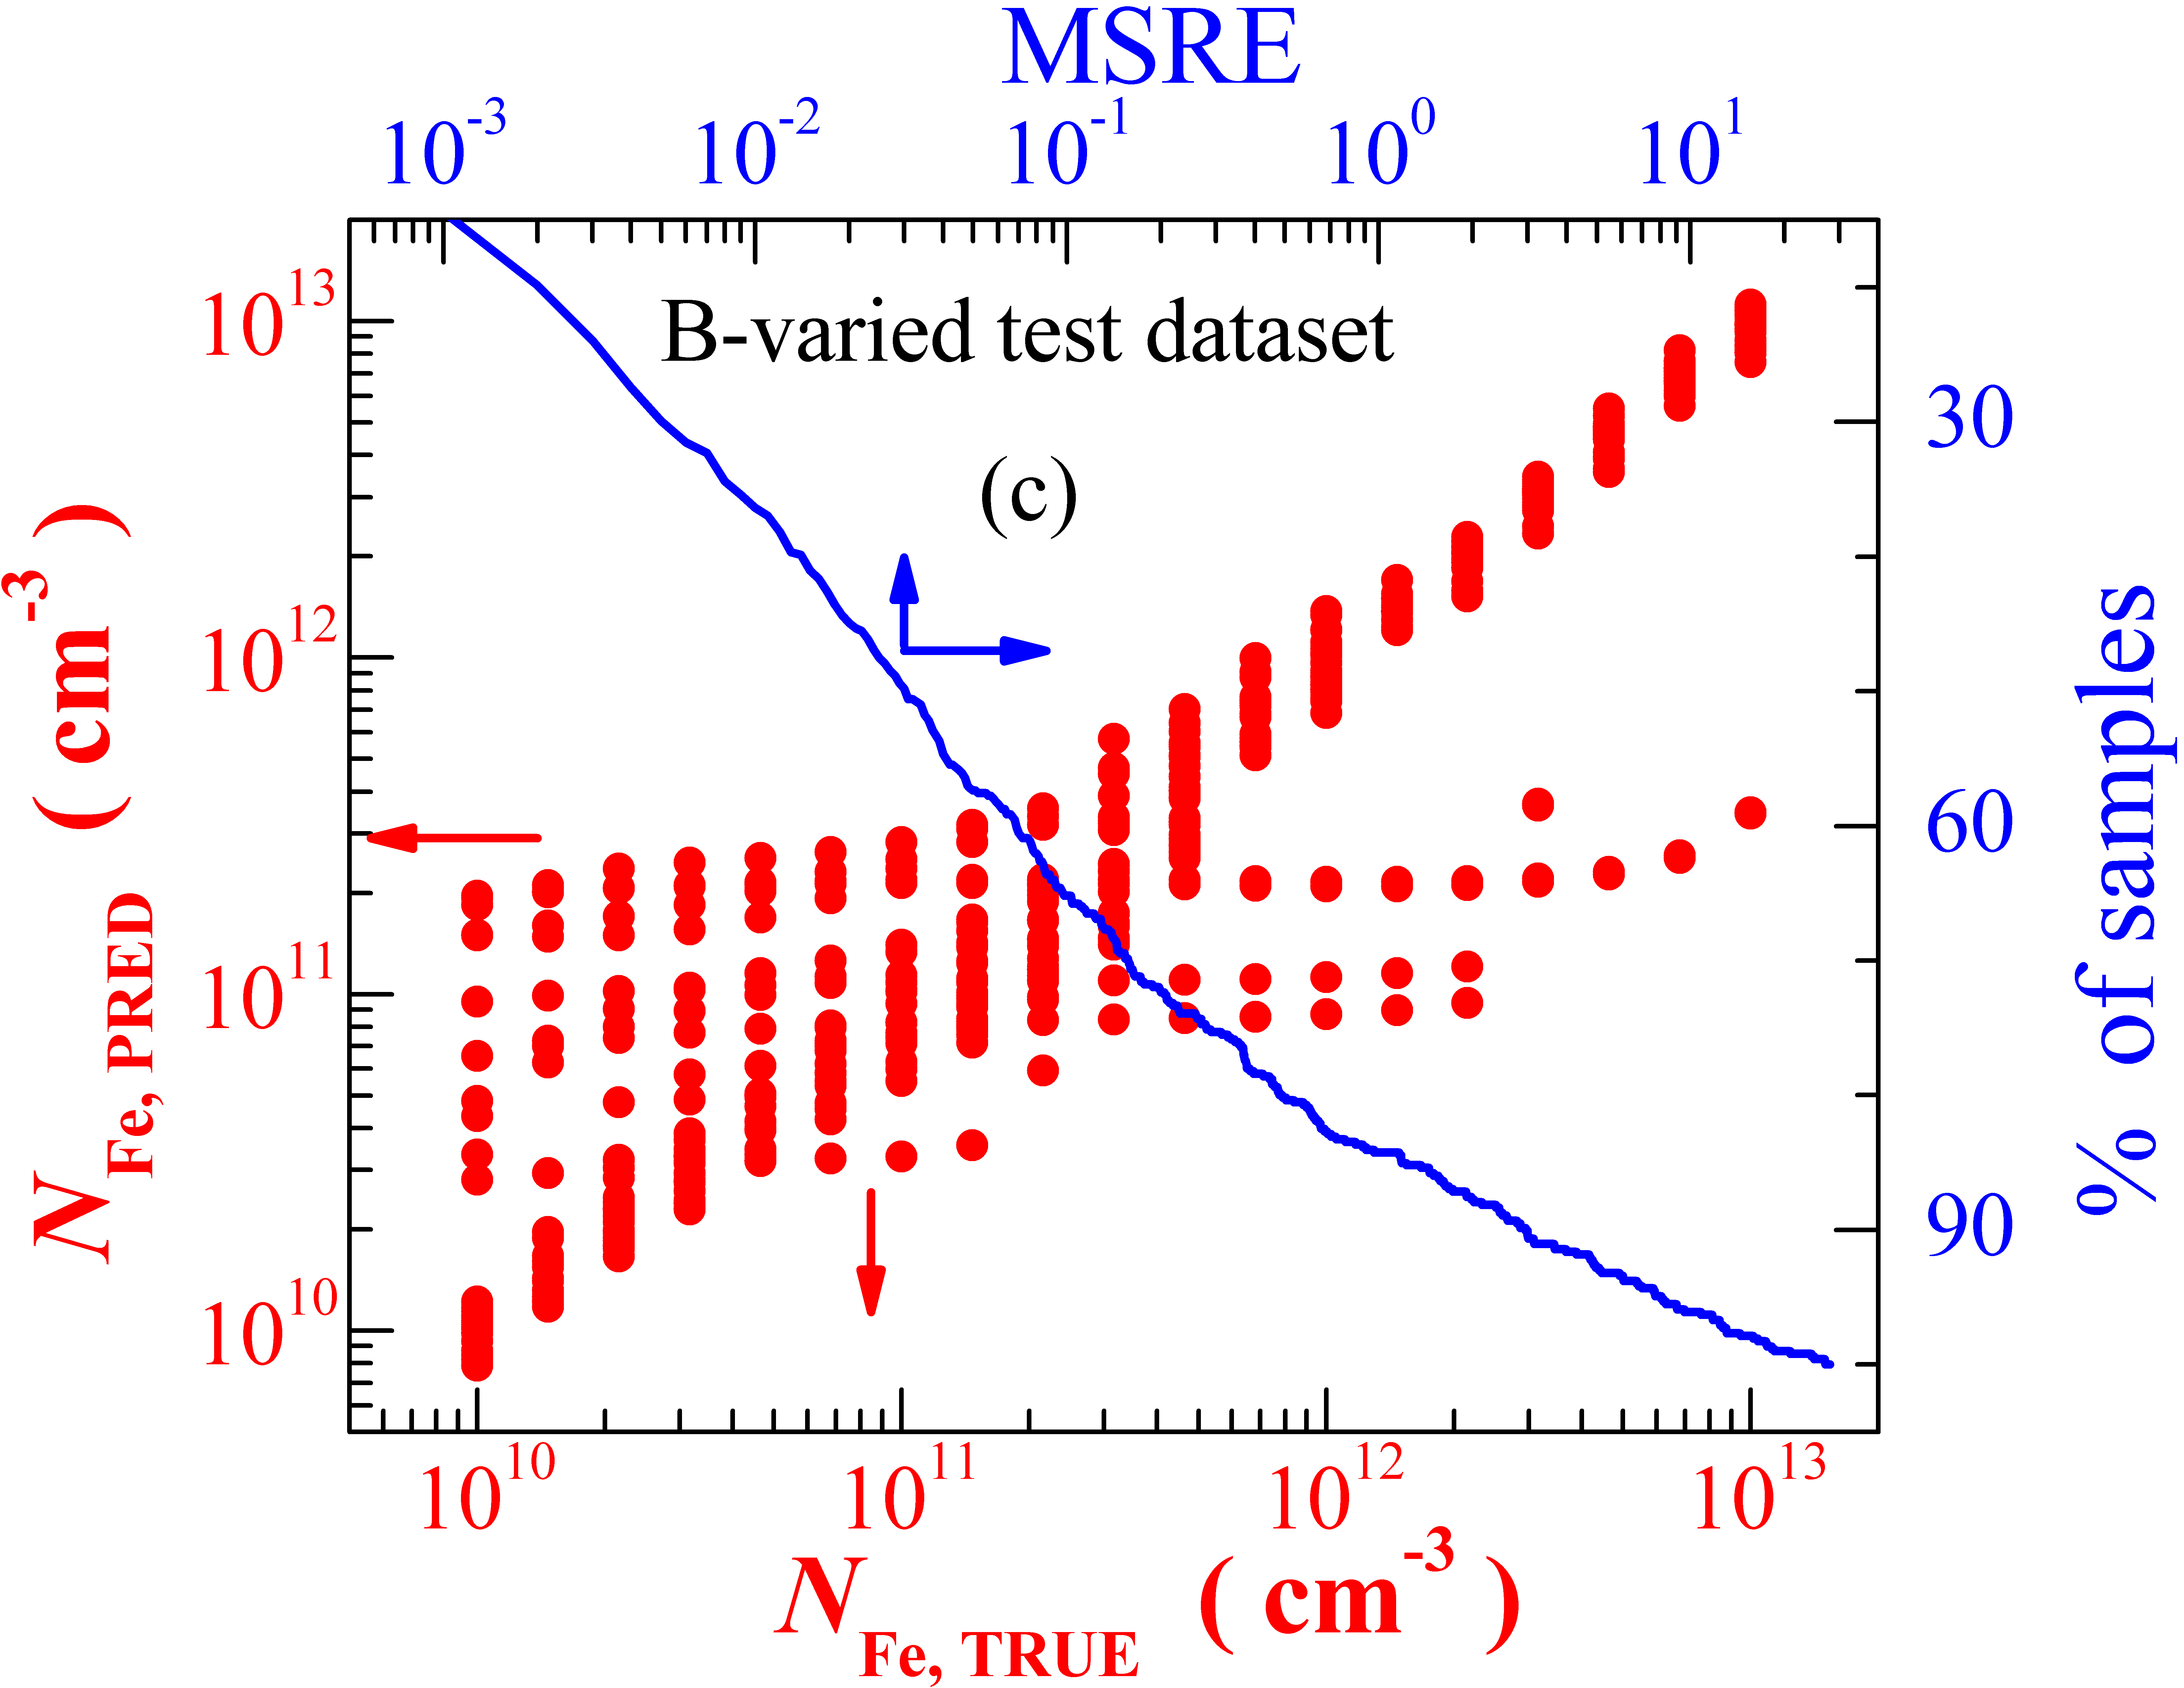
\includegraphics[width=0.32\textwidth]{Fig2d}

\includegraphics[width=0.32\textwidth]{Fig2e}
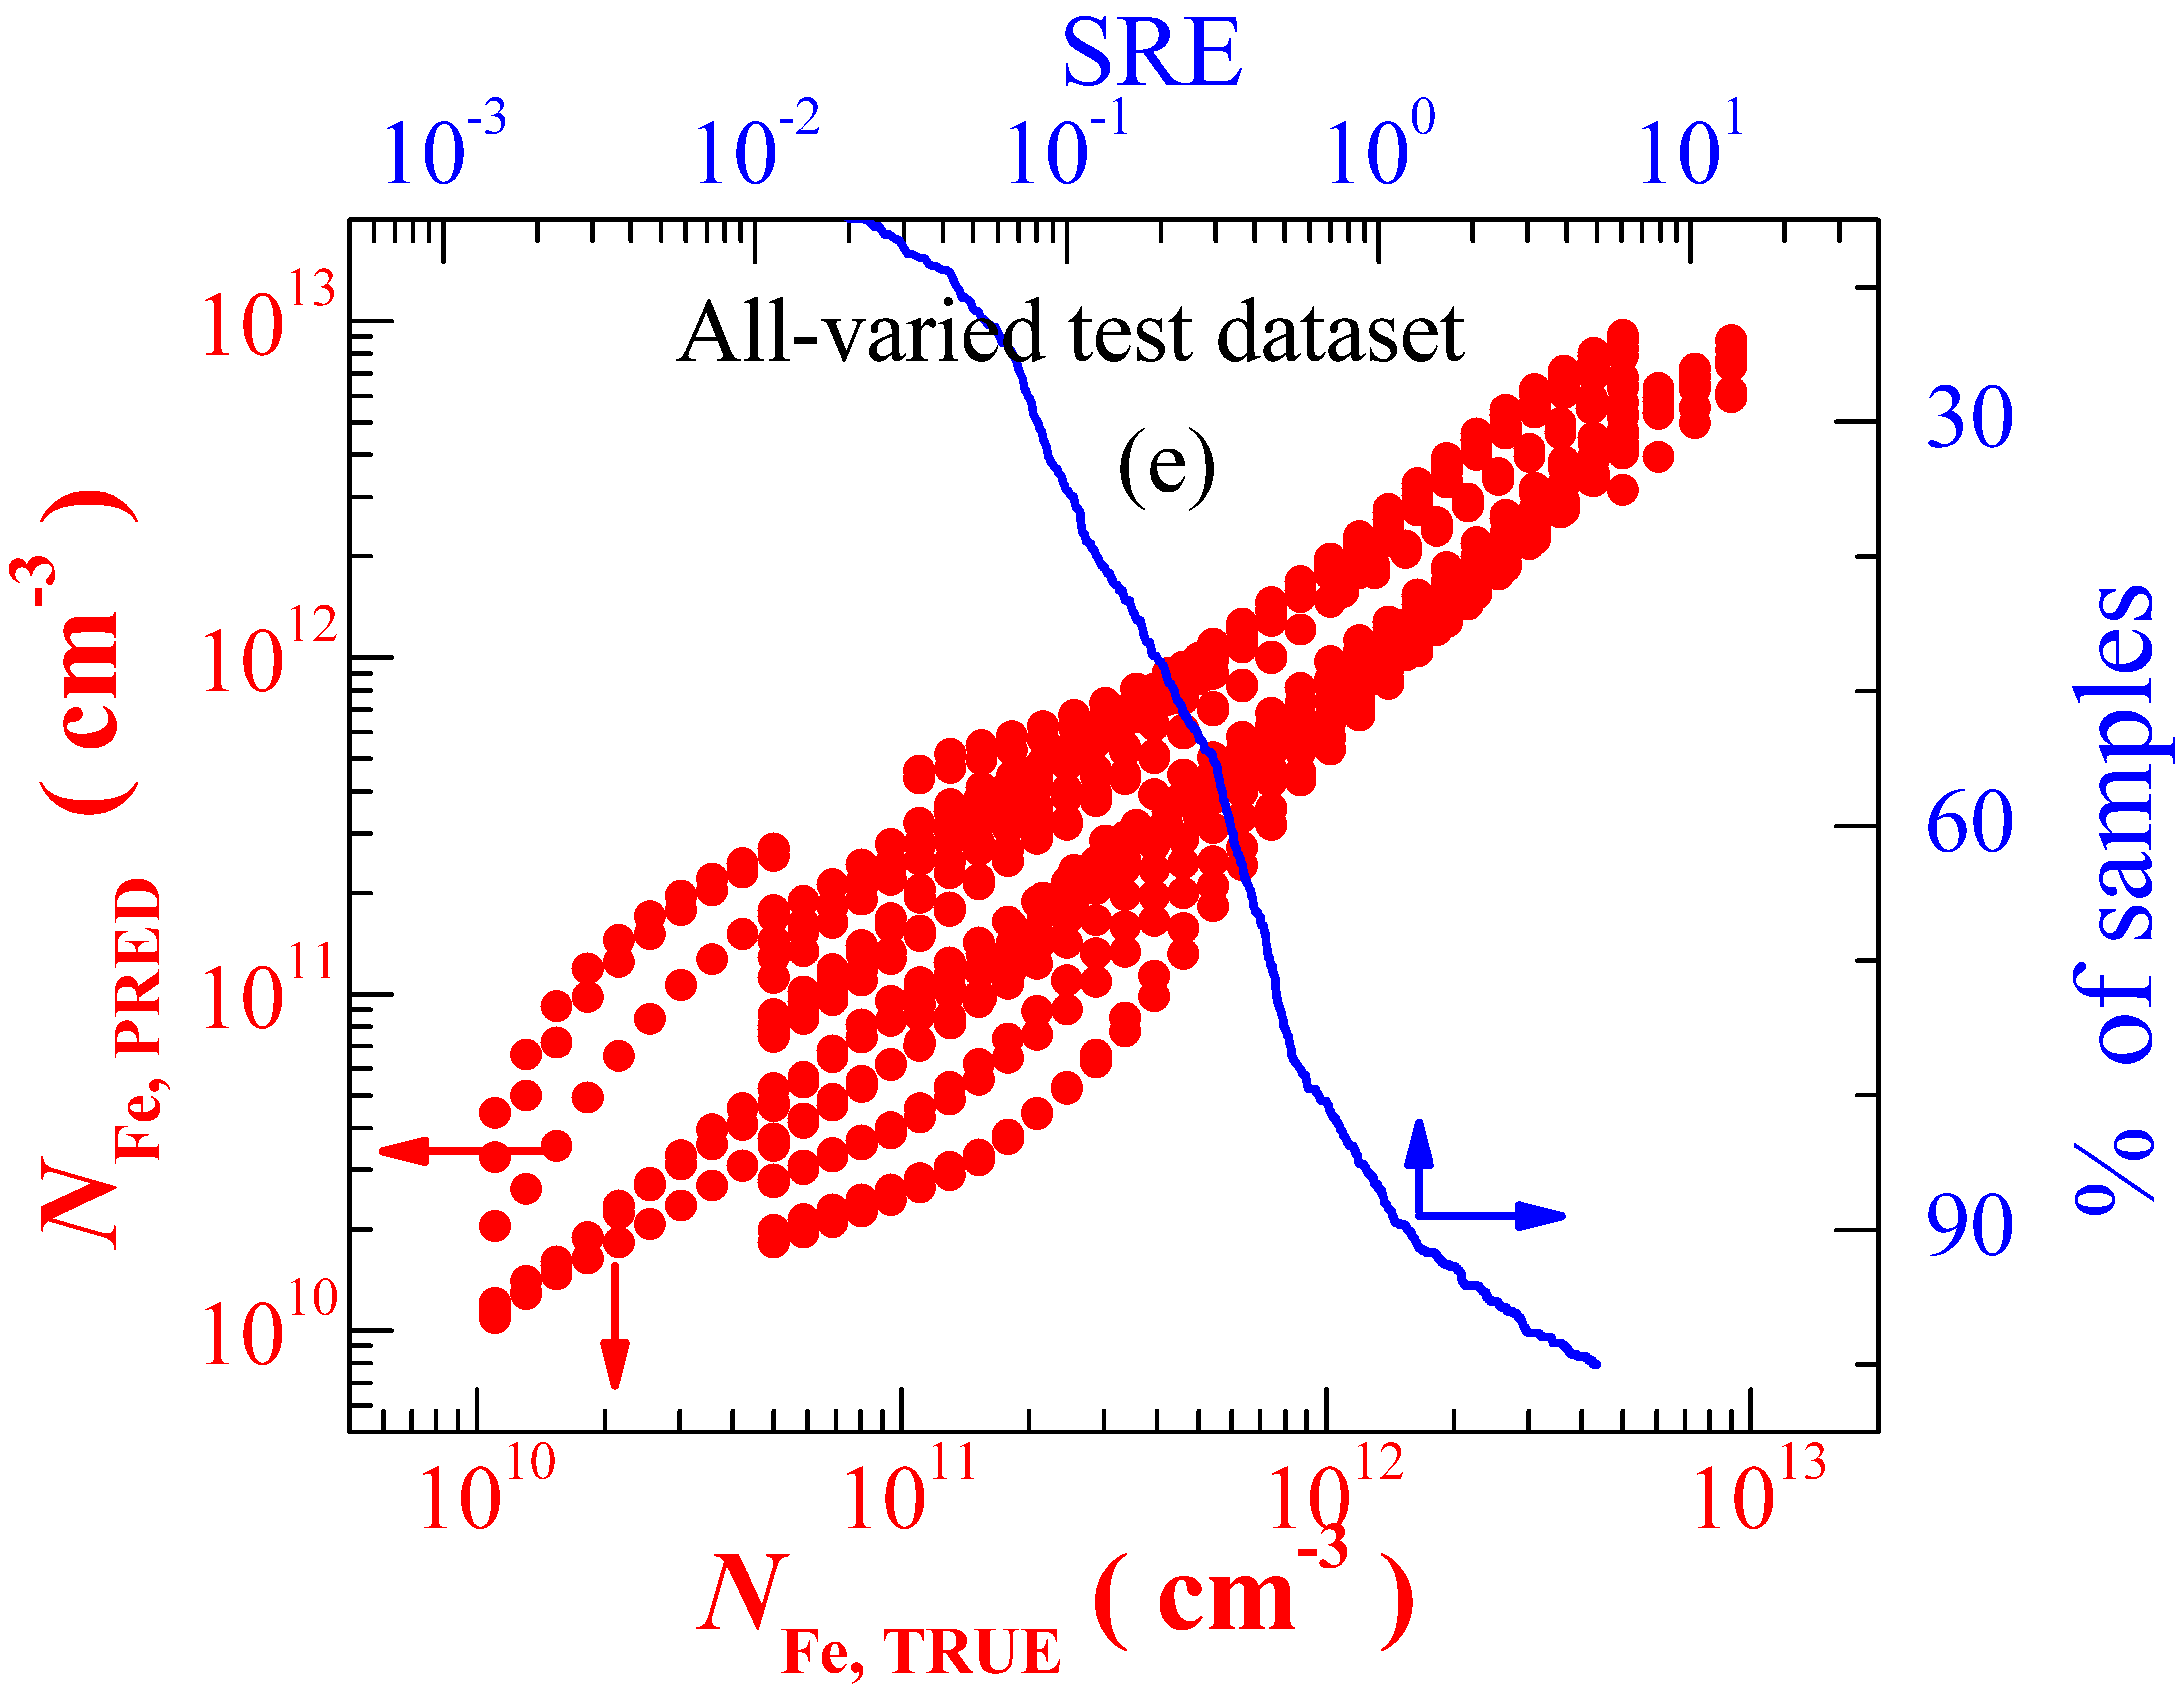
\includegraphics[width=0.32\textwidth]{Fig2f}
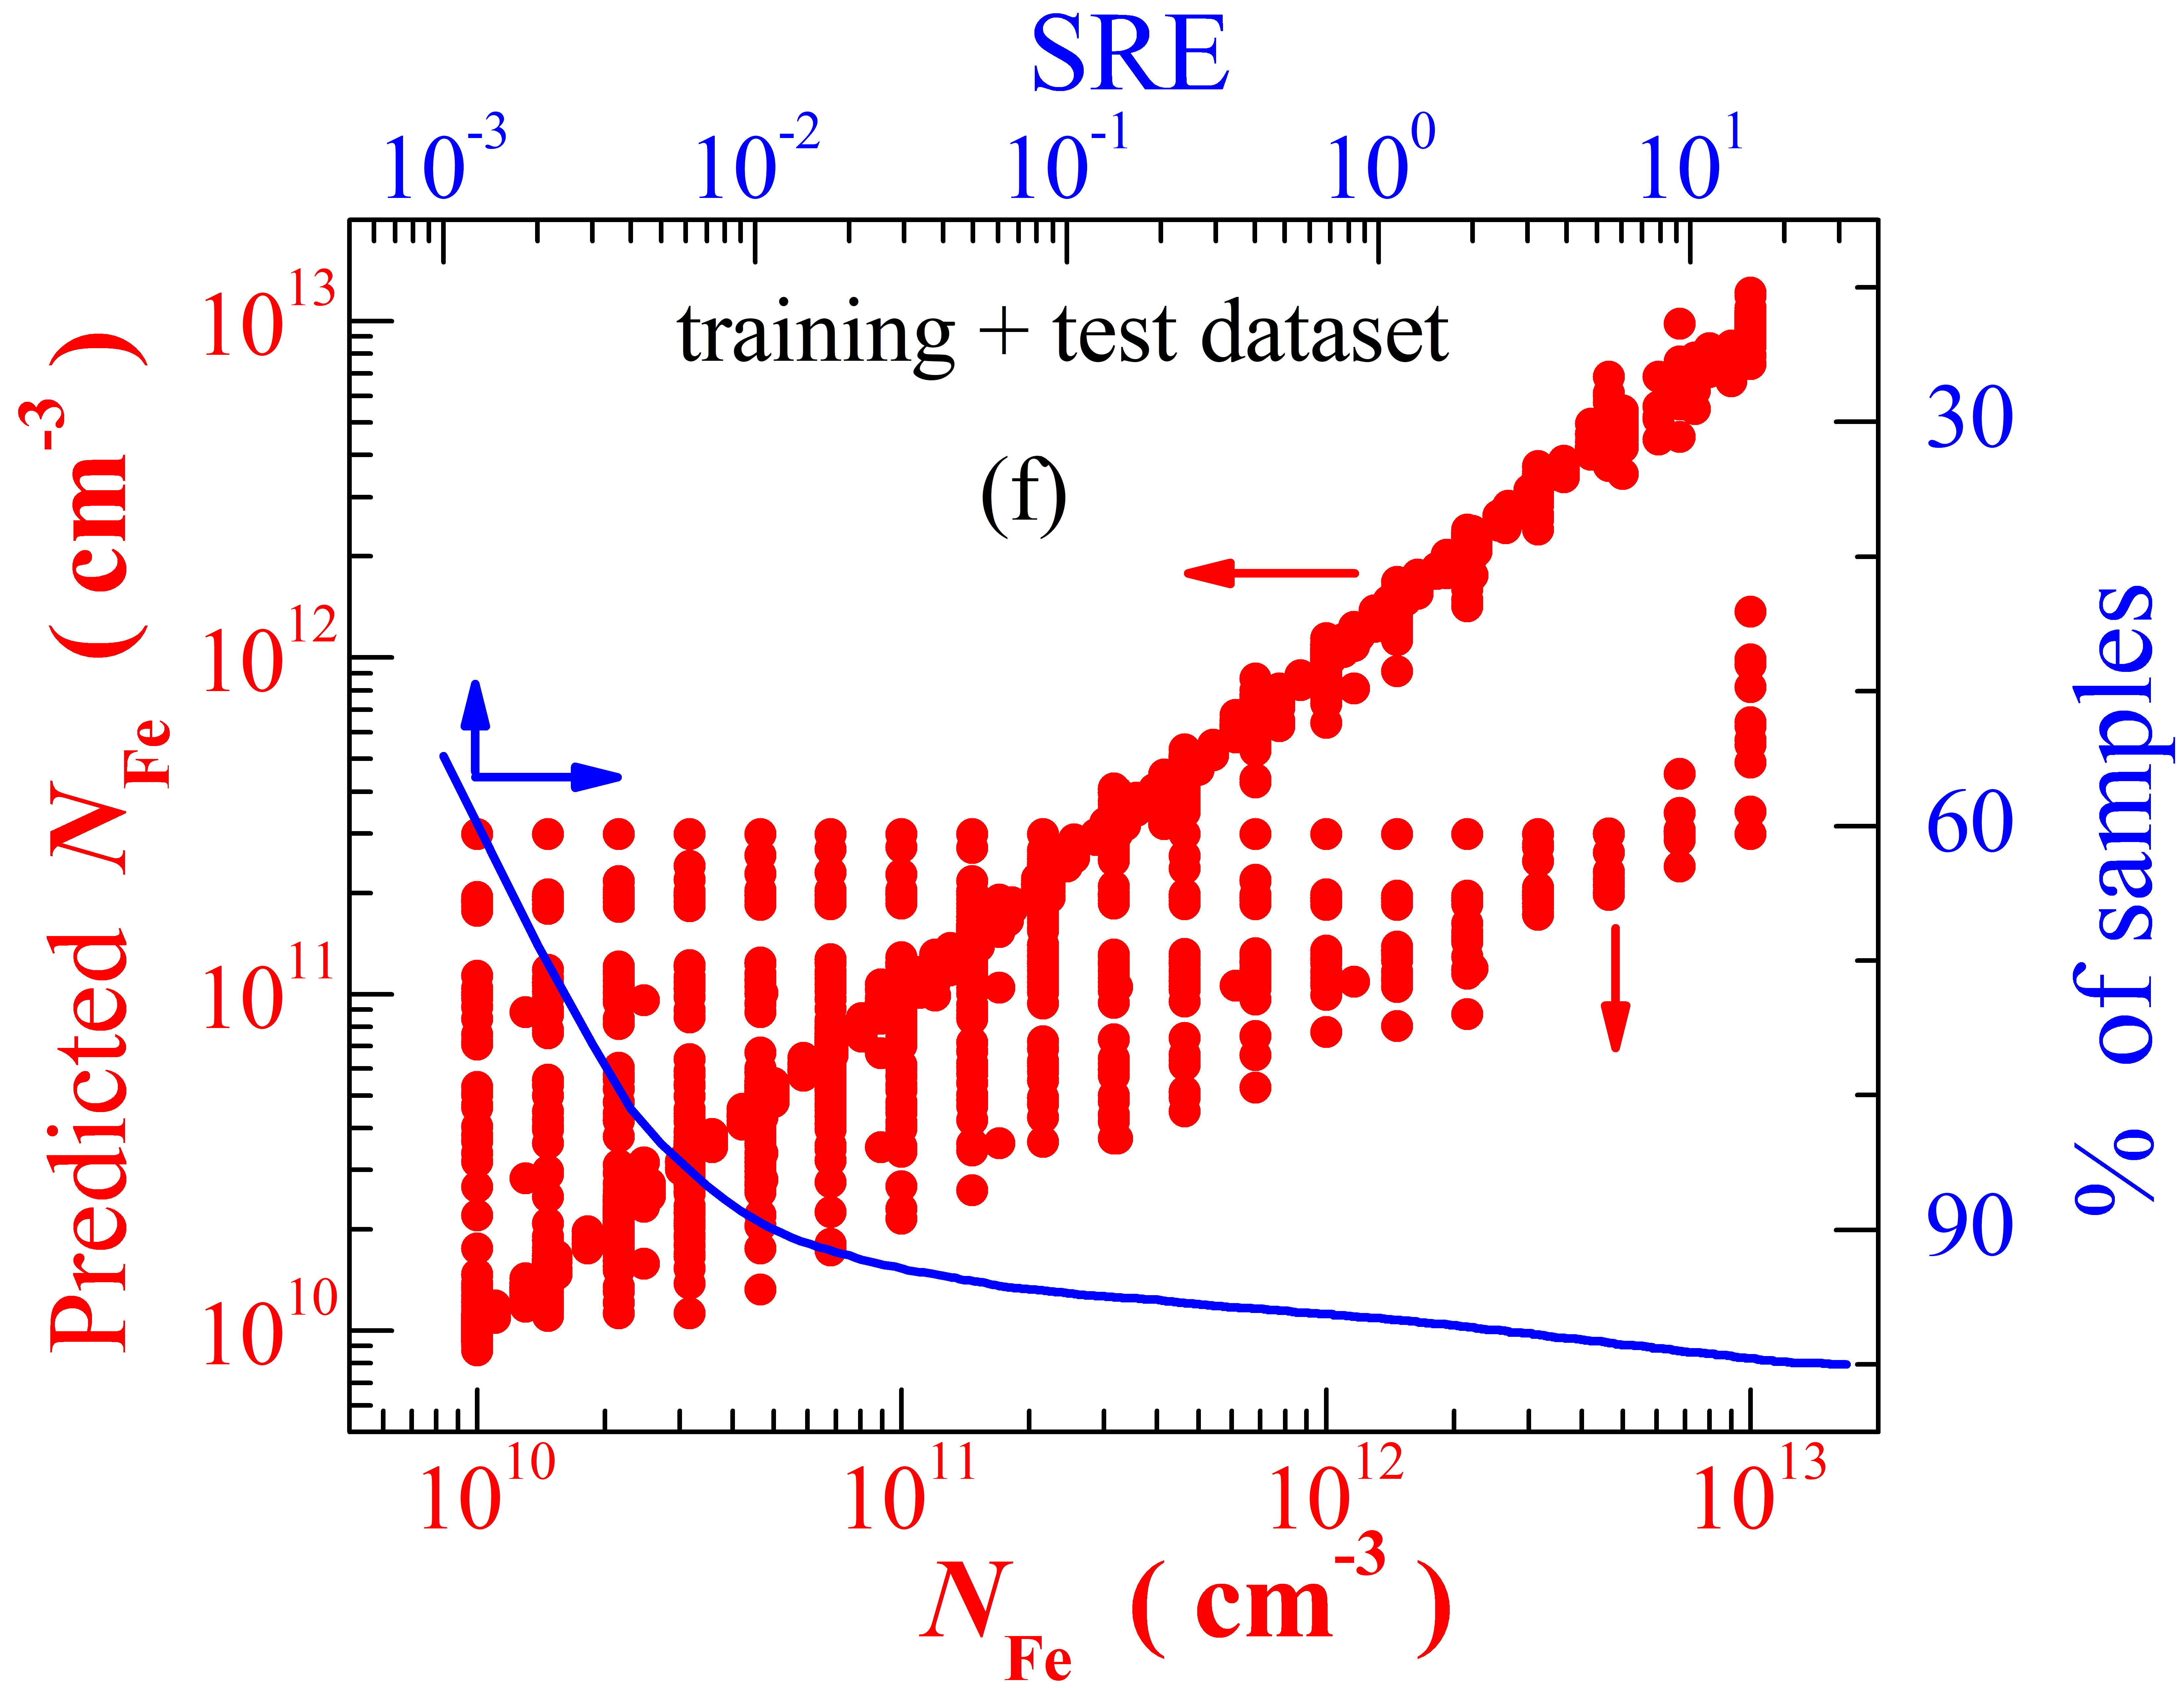
\includegraphics[width=0.32\textwidth]{Fig2g}
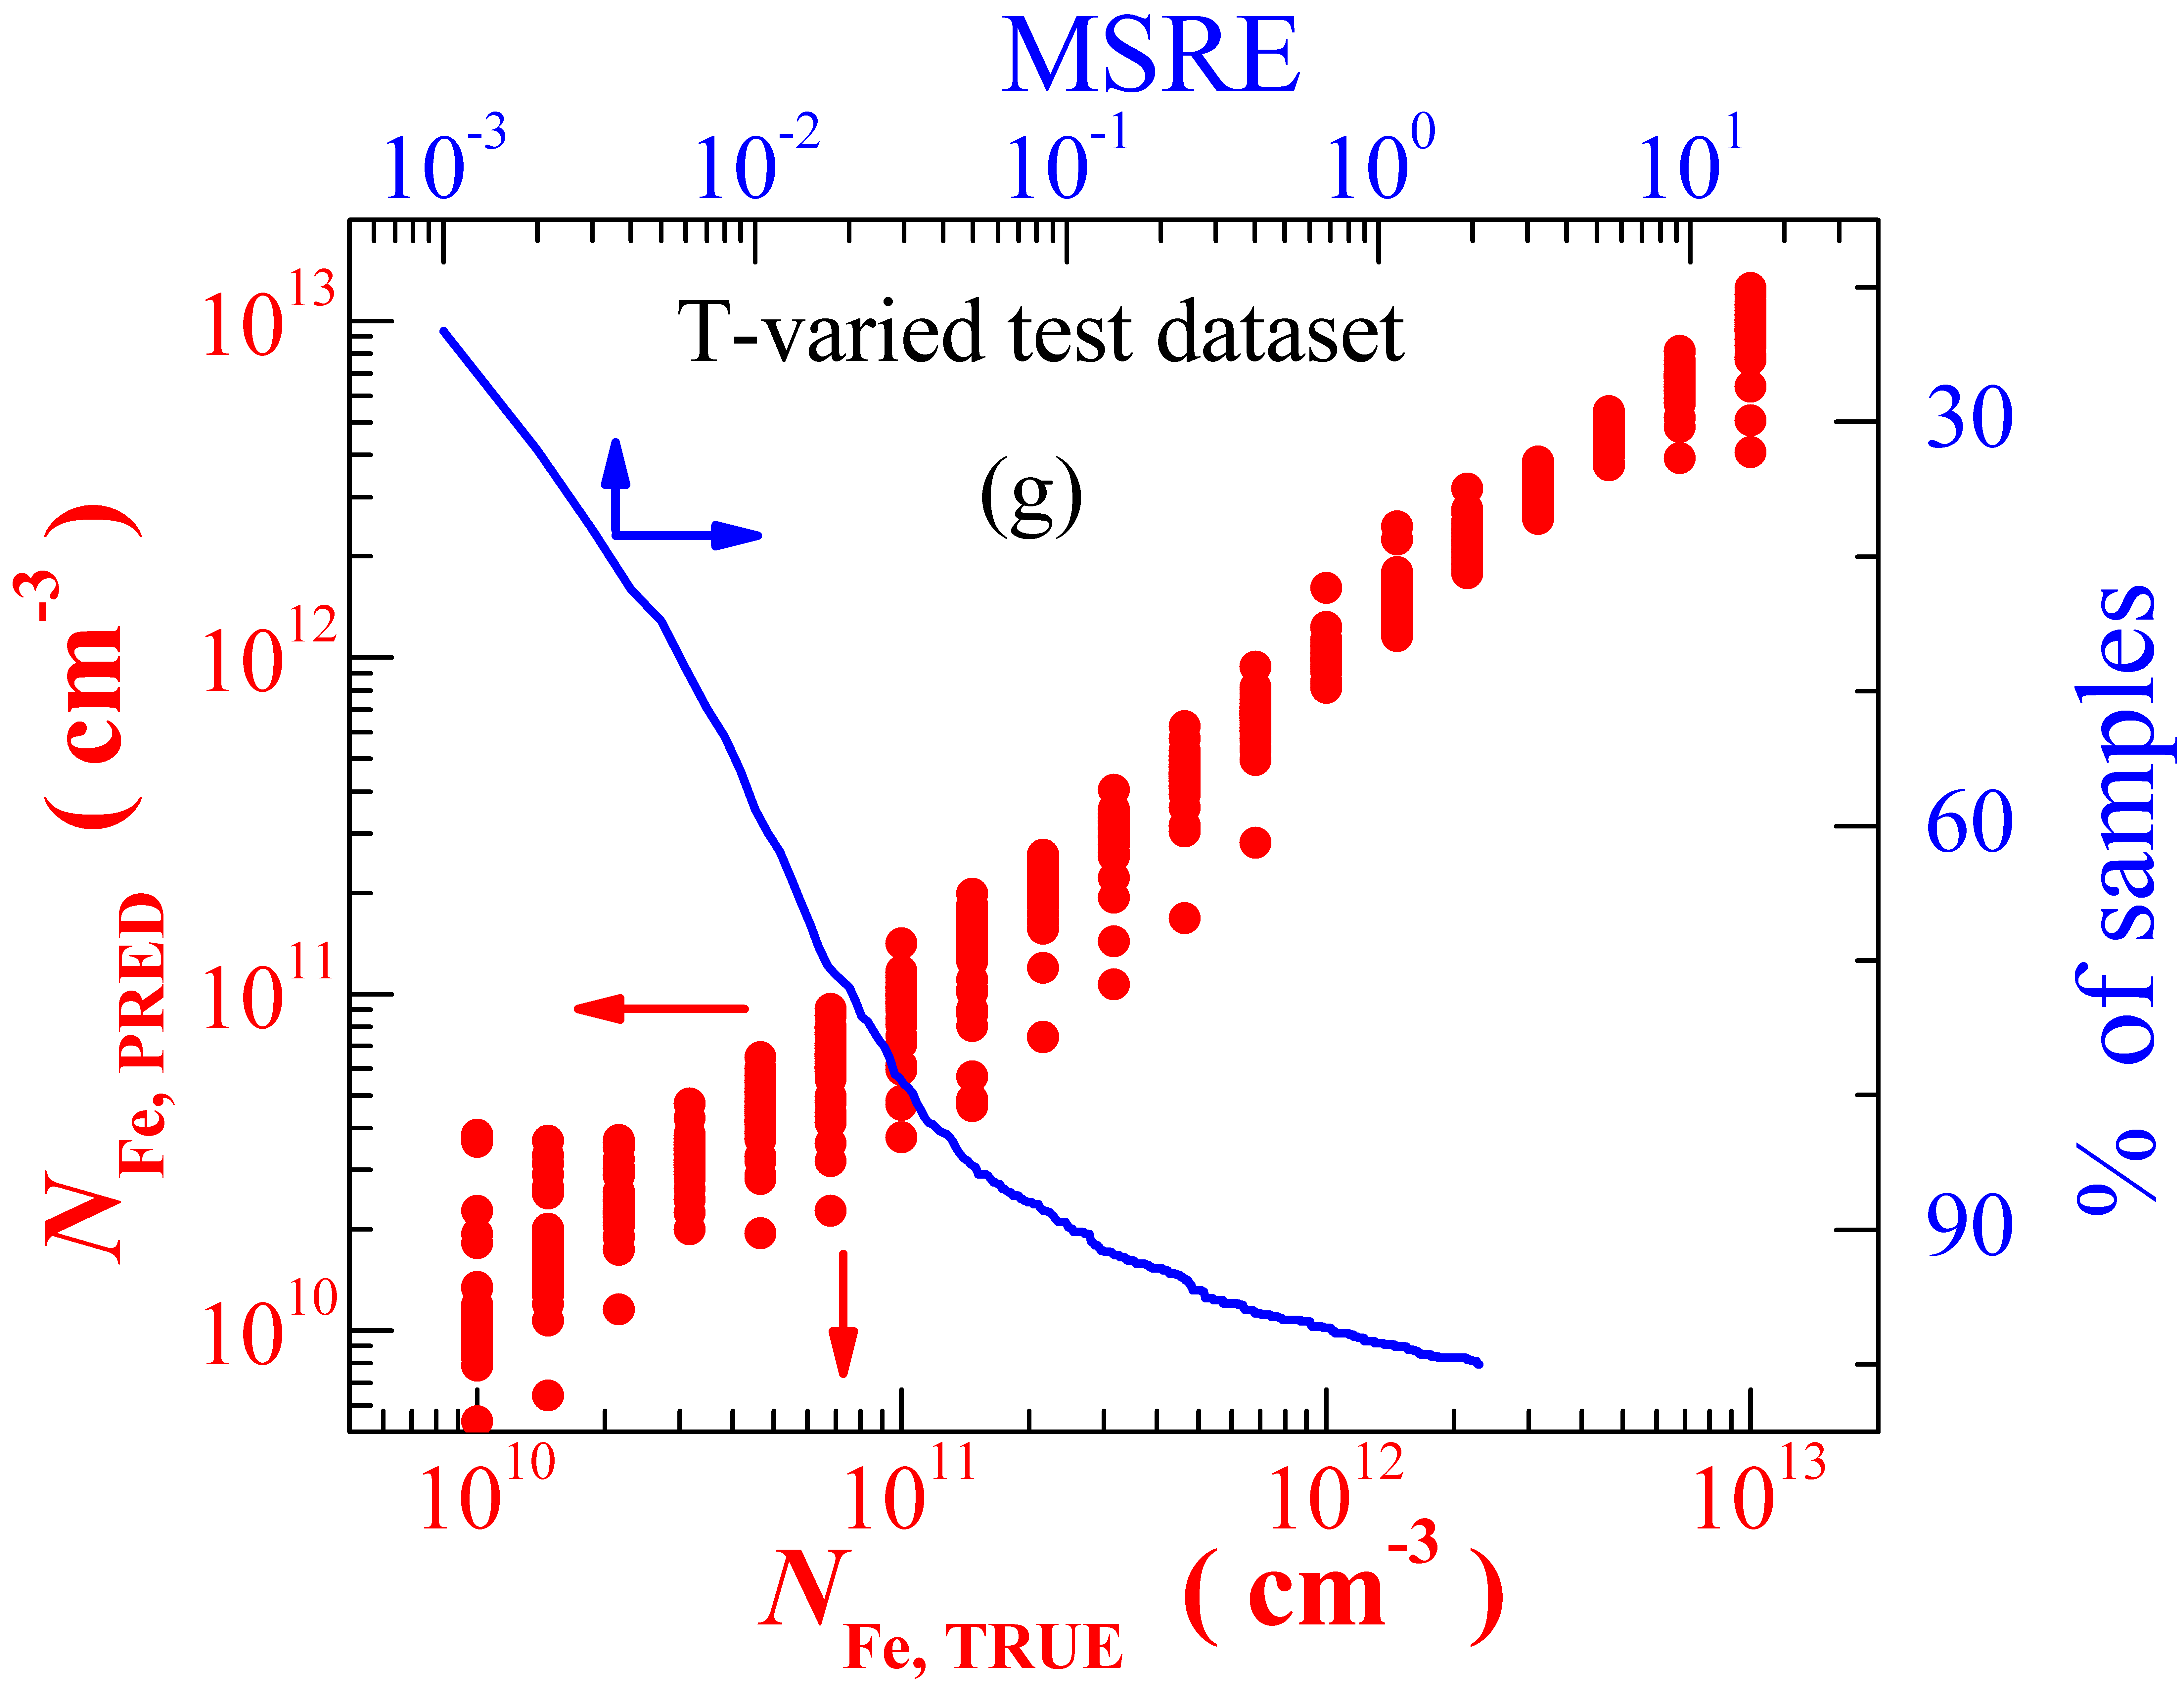
\includegraphics[width=0.32\textwidth]{Fig22b}

\includegraphics[width=0.32\textwidth]{Fig22c}
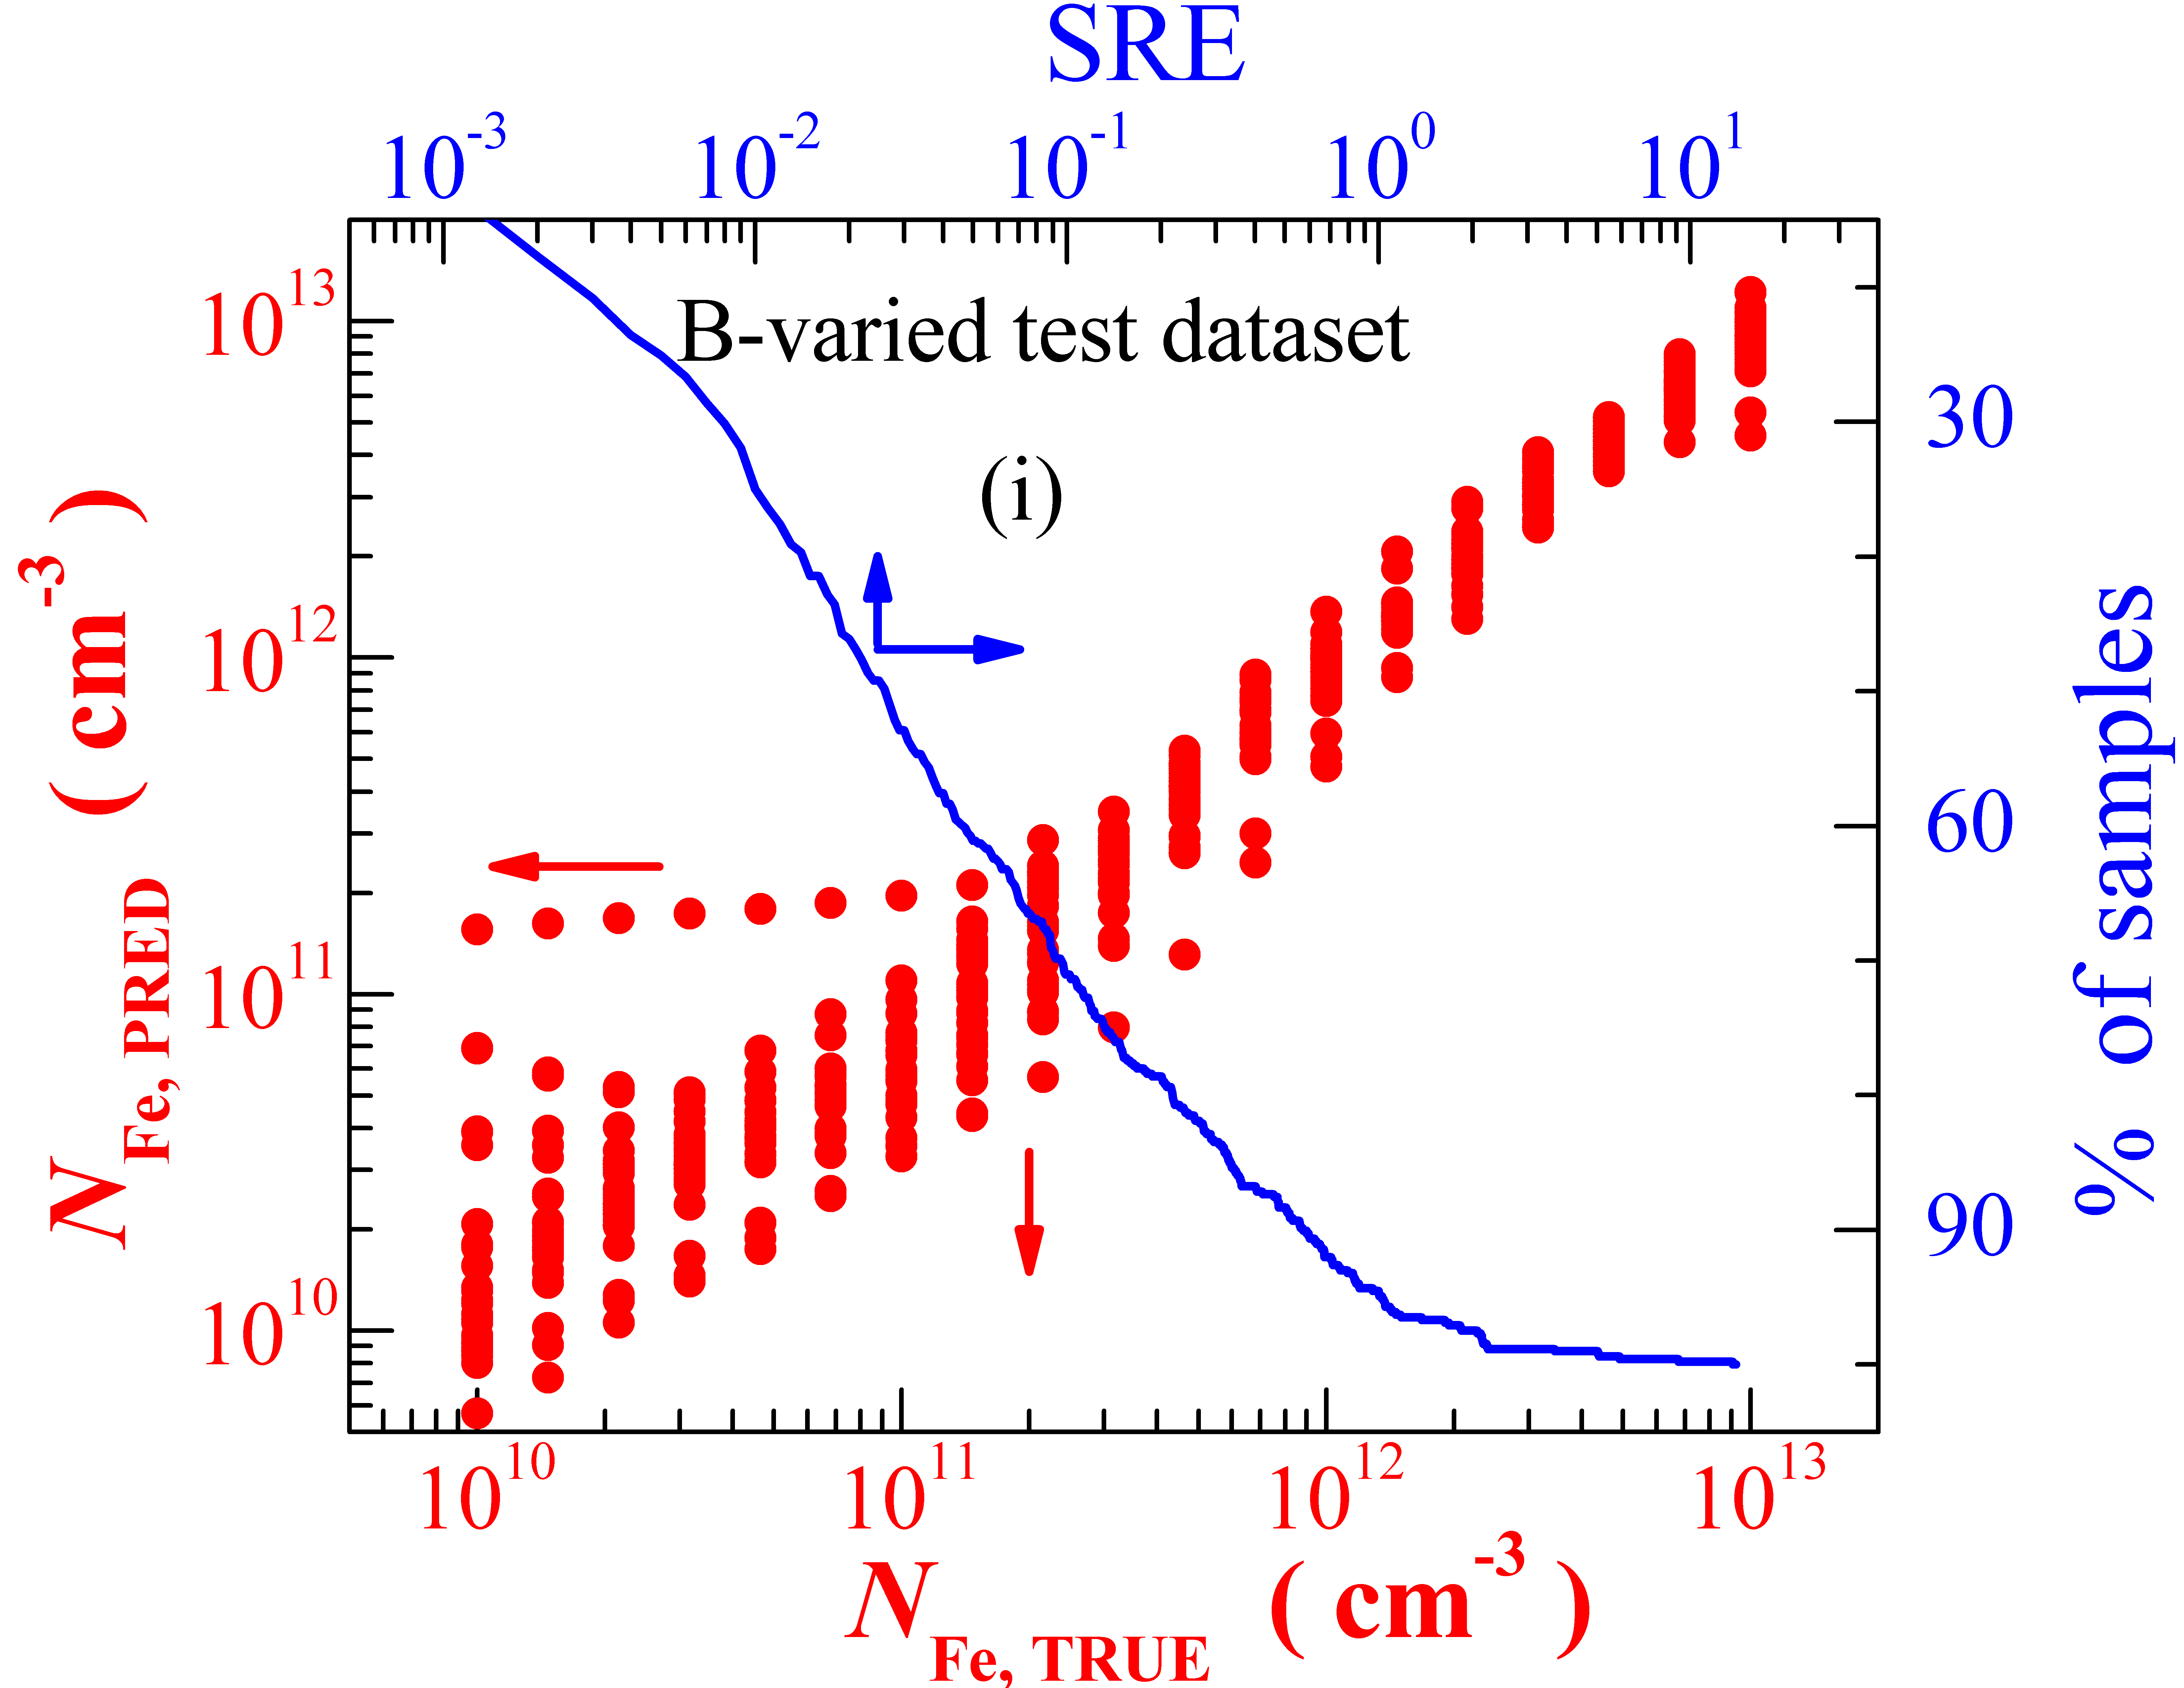
\includegraphics[width=0.32\textwidth]{Fig22d}
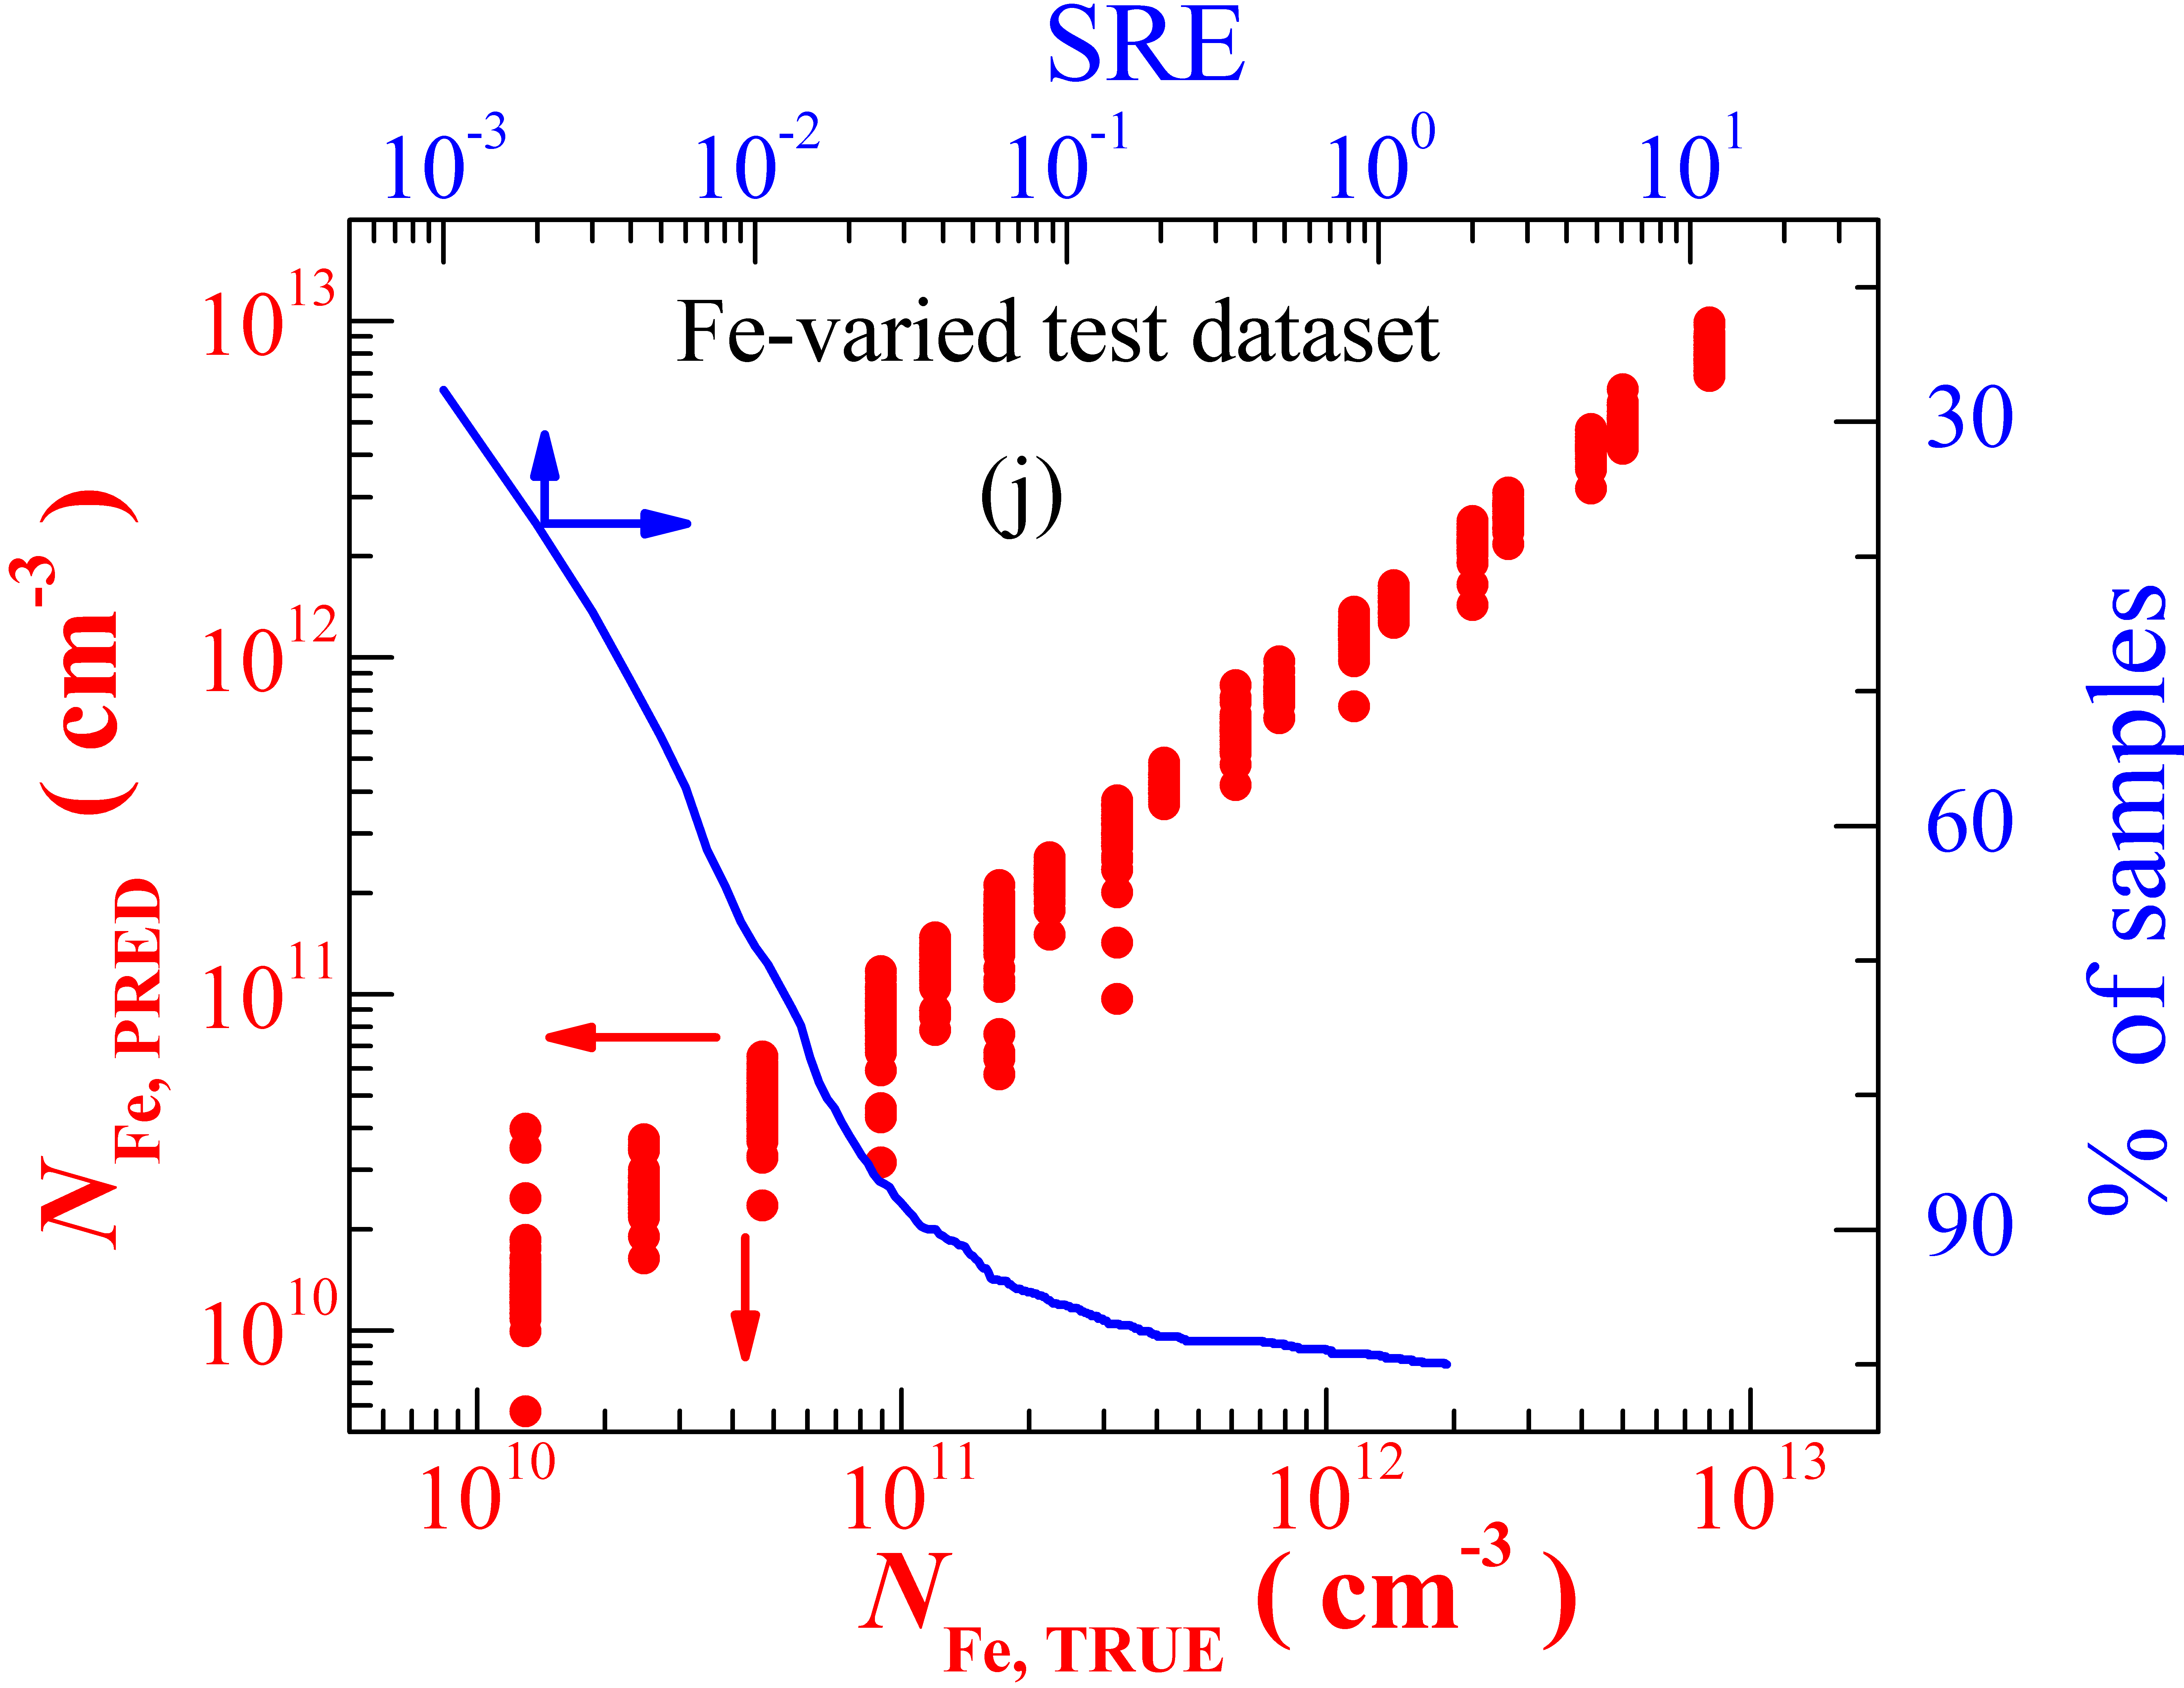
\includegraphics[width=0.32\textwidth]{Fig22e}

\includegraphics[width=0.32\textwidth]{Fig22f}

\includegraphics[width=0.32\textwidth]{Fig22g}
\caption{Comparison of iron contamination retrieval results (red points)
and part of samples with SRE not exceeding a certain value (blue lines).
$n_\mathrm{Fe-FeB}$ DNN and $n_\mathrm{Fe-FeB}$--$n_\mathrm{Fe}$ DNN were used
in panels (a)--(f) and (g)--(l), respectively.
Test dataset: T-varied (a, g),
d-varied (b, h),
B-varied (c, i),
Fe-varied (d, j),
All-varied (e, k).
DNNs were trained by training dataset ((a)--(e), (g)--(k))
or full (f, l) dataset.
%Panels (f) and (l) represent results of  data from
%$n_\mathrm{Fe-FeB}$ DNN and $n_\mathrm{Fe-FeB}$--$n_\mathrm{Fe}$ DNN,
%which learnt by training+test dataset, on  the same dataset.
}
\label{fig_TrPr}
\end{figure*}

The one-parameters divergence in other cases from training magnitude has not vital importance:
the $N_\mathrm{Fe,TRUE}$ and $N_\mathrm{Fe,PRED}$ difference can be occasionally significant,
but SRE for about 80 percent of the samples does not exceed 0.01 in cases of T-varied and d-varied dataset --- see Fig.~\ref{fig_TrPr}(a),(b).
At the same time, the predictive power of the $n_\mathrm{Fe-FeB}$ DNN is very limited in the All-varied dataset:
the SRE is less than 0.1 in 30 percent of cases only.

It is obviously, that $n_\mathrm{Fe-FeB}$ DNN  properties can can be improved by a configuration tuning as well as an extension in training dataset.
But in our opinion, the network predictive ability is fundamentally limited by $n_\mathrm{Fe-FeB}$ vs $N_\mathrm{Fe}$ dependence ambiguity (see details elsewhere \cite{OlikhJPS}).
The increase in the input parameter number is quite expected to enhances the DNN capability.
But the expected improvement of the $n_\mathrm{Fe-FeB}$--$n_\mathrm{Fe}$ DNN must be also caused by the removal of a certain degeneration of correlation between an ideality factor value and an iron concentration (a kind of splitting).

Indeed, one can see the improvement in operating characteristic
of $n_\mathrm{Fe-FeB}$--$n_\mathrm{Fe}$ DNN in comparison with $n_\mathrm{Fe-FeB}$ DNN.
The improvement manifests itself both in the MSRE decrease (see Table~\ref{table_MSRE}) and
in the almost complete absence of huge
difference in $N_\mathrm{Fe,TRUE}$ and $N_\mathrm{Fe,PRED}$ values.
Really, the maximum SRE does not exceed 1 and SRE is less than 0.1 for 60\% of samples
even for the All-varied test dataset --- see Fig.~\ref{fig_TrPr}(k).

Despite the difference in predicting accuracy,
the $n_\mathrm{Fe-FeB}$--$n_\mathrm{Fe}$ DNN's features are similar to  $n_\mathrm{Fe-FeB}$ DNN's ones.
Thus difference in $N_\mathrm{B}$ value from training dataset is the most troublesome case
(Fig.~\ref{fig_TrPr}(i)).
The enjoyable (from a practical point of view) attribute is an ability to predict iron concentration value, which not used under learning.

It is known \cite{Keras} that the increase of labeled dataset to train on leads to improve  deep neural network results.
We have used all simulated data (so-called full dataset) to train both
$n_\mathrm{Fe-FeB}$--$n_\mathrm{Fe}$ DNN and $n_\mathrm{Fe-FeB}$ DNN as well.
The results are presented in Table~\ref{table_CV} and Fig.~\ref{fig_TrPr} (f) and (l).
Surprisingly the expansion of training base did not make better the results of cross--validation
for $n_\mathrm{Fe-FeB}$ DNN.
In our opinion, the mentioned above features of $n_\mathrm{Fe-FeB}$ vs $N_\mathrm{Fe}$ dependence
are a reason of such result.
At the same time the increase in number of samples leds to essential raise trainability of network, which uses two ideality factor value.


%from sklearn.model_selection import cross_val_score
%https://github.com/olegolikh/IVcharacteristics.git


%\begin{equation}
%\label{eqn_Eg}
%E_g(T) = E_g(0)-\alpha\,\theta\left\{\frac{1-3\Delta^2}{\exp{(\theta/T)}-1}+
%  \frac{\theta^2}{2}\left(\sqrt[6]{1+\frac{\pi^2}{3(1+\Delta^2)}\left(\frac{2T}{\theta}\right)^2
%  +\frac{3\Delta^2-1}{4}\left(\frac{2T}{\theta}\right)^3+\frac{8}{3}\left(\frac{2T}{\theta}\right)^4
%  +\left(\frac{2T}{\theta}\right)^6}-1\right)\right\},
%\end{equation}
%
%\setlength{\arraycolsep}{0.0em}
%\begin{eqnarray}
%Z&{}={}&E_g(0)-\alpha\,\theta\left\{\frac{1-3\Delta^2}{\exp{(\theta/T)}-1}\right\}\nonumber\\
%&&+\frac{\theta^2}{2}\left(\sqrt[6]{1+\frac{\pi^2}{3(1+\Delta^2)}\left(\frac{2T}{\theta}\right)^2
%  +\frac{3\Delta^2-1}{4}\left(\frac{2T}{\theta}\right)^3+\frac{8}{3}\left(\frac{2T}{\theta}\right)^4
%  +\left(\frac{2T}{\theta}\right)^6}-1\right)
%\end{eqnarray}
%\setlength{\arraycolsep}{5pt}

%\hfill mds

%\hfill August 26, 2015


The results on IVC simulation, $n_\mathrm{Fe}$ and $n_\mathrm{Fe-FeB}$ values
and trained DNNs are presented at \emph{https://github.com/olegolikh/IVcharacteristics.git}.

\section{Conclusion}

In this work, we demonstrate the ability to extract impurity contamination
from IV measurements (an ideality factor value) and utilizing a deep neural network.
These approach utilizes a simple and widely applicable setup and
does not require a much experimental time.

The method is based on the ability to train the deep neural network by using the
results of simulation of solar cell with various parameters, in particular, the impurity concentration.
In this model study, we investigated a single crystal silicon $n^+$--$p$--$p^+$ system with iron for which parameters have been extensively reported in the literature.
The obtained results show that the dense layer DNN, trained with structure base doping level value and thickness, is able to predict iron concentration with MSRE up to 0.03 by using ideality factor values.
The analysis has shown that it is important to train DNN by boron concentration value of structure under consideration.
It is likely that two ideality factor values (for structure with $\mathrm{Fe}_i$ only as well as with $\mathrm{Fe}_i\mathrm{B}_s$ and $\mathrm{Fe}_i$ coexistence) would be needed to substantially upgrade a prediction accuracy.

Furthermore, IV measurement is a standard SC characterization technique,
meaning this approach could be integrated into manufacturing environment.


%The relationship between the diode ideality factor and the iron concentration in the base layer of silicon $n^+-p$ solar cells has been studied via computer simulation.
%The data used in the simulations were the following.
%The iron concentration ranged from $10^{10}$ to $10^{13}$~cm$^{-3}$,
%the base doping level --- from $10^{15}$ to $10^{17}$~cm$^{-3}$,
%and the temperature --- from $290$ to $340$~K.
%The obtained results show that the ideality factor value can be used to estimate the contaminant concentration.
%In particular, the analysis has shown that in case of the Shockley--Read--Hall recombination and the unpaired interstitial iron, it is sufficient to measure single $I-V$ characteristic measurement and find single ideality factor value to evaluate iron concentration.
%If the Auger recombination, radiative recombination, or iron--boron pair presence has to be taken into account,
%then the measurements over a temperature range are necessary.
%For these cases, we have calculated the calibration curves and suggested analytic expressions.


% use section* for acknowledgment
\section*{Acknowledgment}

%The authors would like to thank...
The work was supported by National Research Foundation  of Ukraine by the state budget finance
(project 2020.02/0036 "Development of physical base of both acoustically controlled modification and machine learning--oriented characterization for silicon solar cells")

% Can use something like this to put references on a page
% by themselves when using endfloat and the captionsoff option.
\ifCLASSOPTIONcaptionsoff
  \newpage
\fi



% trigger a \newpage just before the given reference
% number - used to balance the columns on the last page
% adjust value as needed - may need to be readjusted if
% the document is modified later
%\IEEEtriggeratref{8}
% The "triggered" command can be changed if desired:
%\IEEEtriggercmd{\enlargethispage{-5in}}


\bibliography{IEEEabrv,olikh}


\begin{IEEEbiography}[{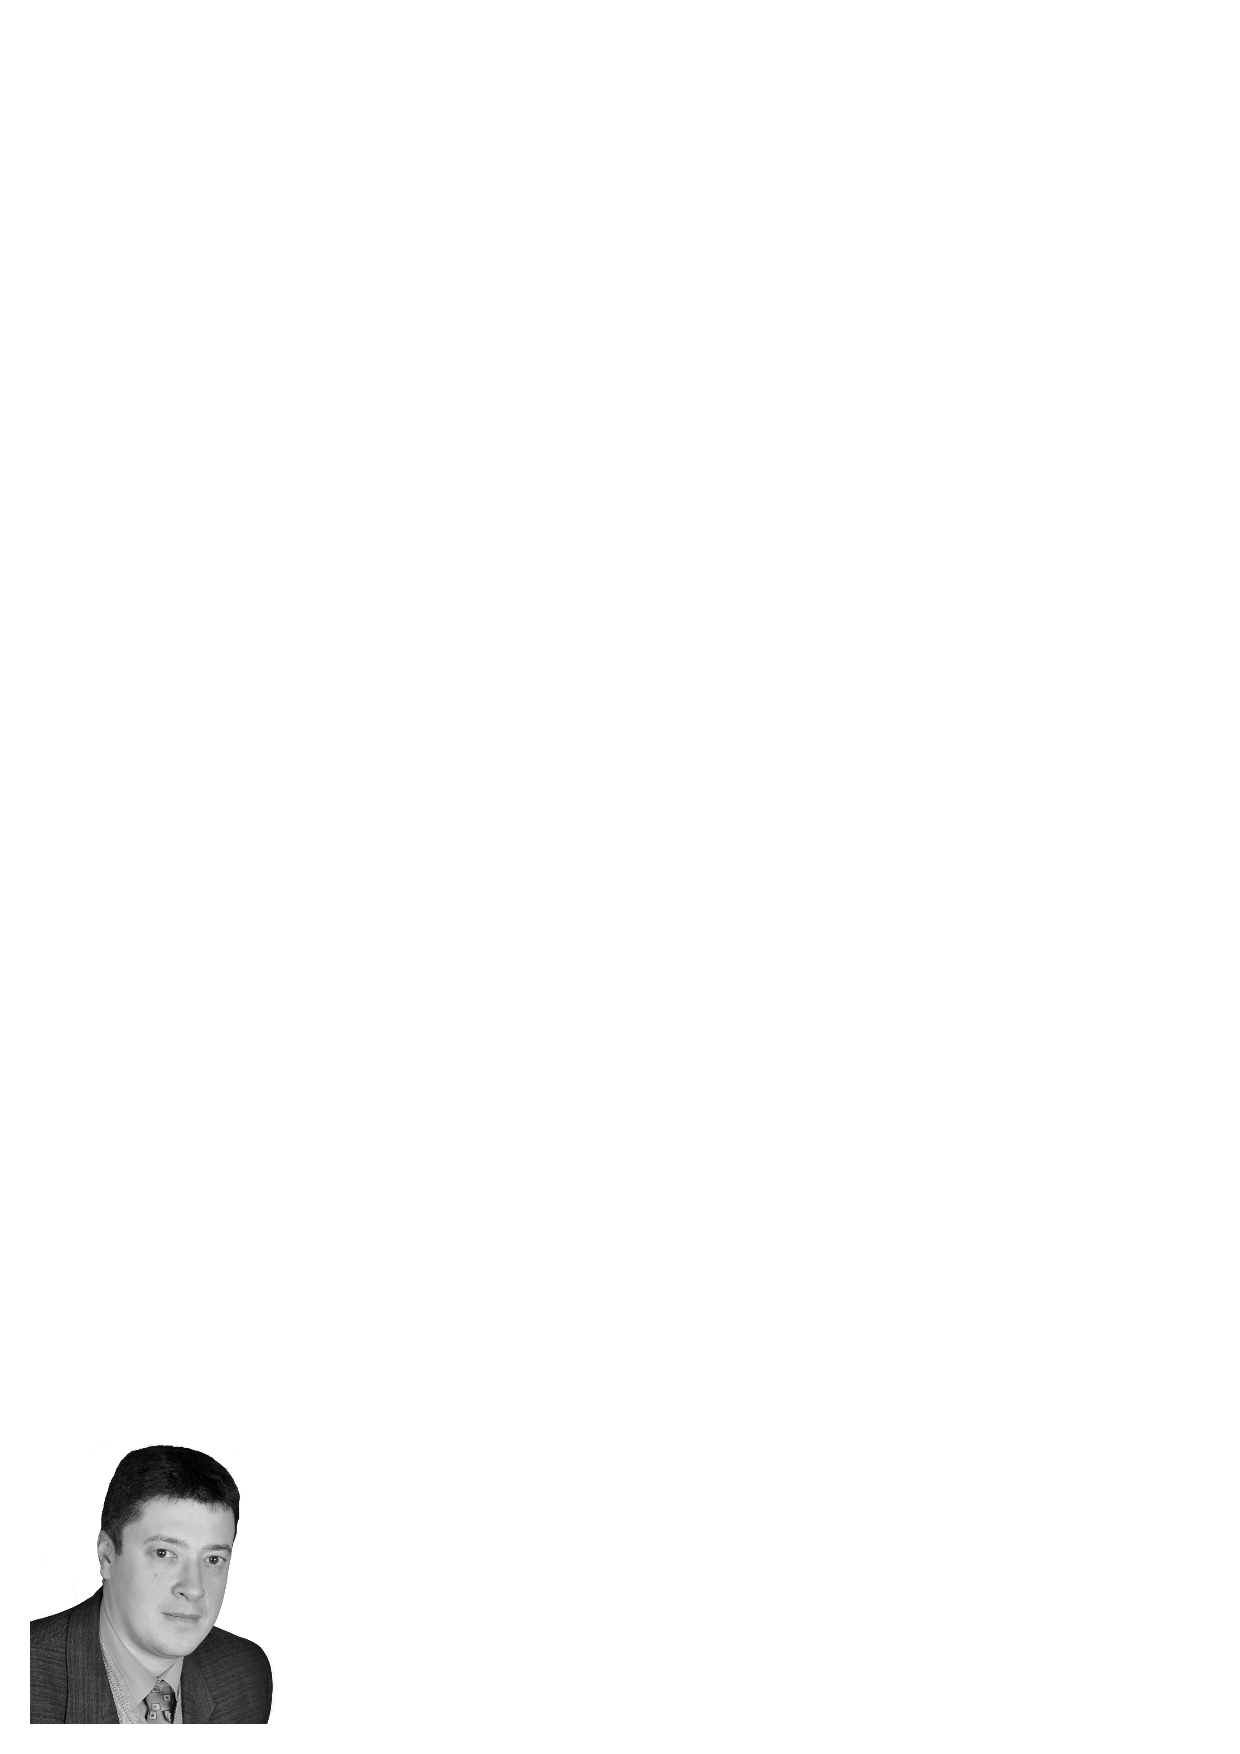
\includegraphics[width=1in,height=1.25in,clip,keepaspectratio]{olikh_foto}}]{Oleg Olikh}
 %Oleg Ya. Olikh
 received the Ph.D. degree in solid state physics at Taras Shevchenko National University of Kyiv,  Ukraine, in 2001, and  D.Sc. degree  in solid state physics at Taras Shevchenko National University of Kyiv, in 2018.
 He is currently an Associate Professor with the Department of General Physics, Taras Shevchenko National University of Kyiv.

 He has been involved in Semiconductor Device research for more than 25 years,
 working on the characterisation of barrier structure, on
 defect acousto-engineering techniques in silicon, and also in
 the field of meta–-heuristic methods.

%Her research interests focus on material
%research in semiconductors, more specifically defect engineering in silicon,
%nanostructured silicon, light-induced degradation, and silicon photodetectors.
%
%
% His research interests in semiconductor physics have focused on external (radiation, ultrasound) influence on properties of semiconductor devices.
\end{IEEEbiography}

% if you will not have a photo at all:
\begin{IEEEbiographynophoto}{Oleg Lozitsky}
received the B.S. and M.S. degree in solid state physics
Taras Shevchenko National University of Kyiv,  Ukraine, in 2015
and in 2017.

He is currently a Graduate Student with Physics Faculty, Taras Shevchenko National University of Kyiv.
His research interests focus on modeling of material physical properties by using machine learning.
\end{IEEEbiographynophoto}

% insert where needed to balance the two columns on the last page with
% biographies
%\newpage

\begin{IEEEbiographynophoto}{Oleksii~Zavhorodnii}
received the B.S. degree in solid state physics
Taras Shevchenko National University of Kyiv,  Ukraine, in 2010.

He is currently studying for a M.S. degree.
His research interests focus on solar cell simulation.
\end{IEEEbiographynophoto}

% You can push biographies down or up by placing
% a \vfill before or after them. The appropriate
% use of \vfill depends on what kind of text is
% on the last page and whether or not the columns
% are being equalized.

%\vfill

% Can be used to pull up biographies so that the bottom of the last one
% is flush with the other column.
%\enlargethispage{-5in}


\end{document}


